\chapter{Interview method}\label{ch.prod_method}

Chapter \ref{ch.var} has introduced the four variables that this thesis focuses on.
On the basis of previous work, it has also broadly divided them into a (comparatively) non-salient\is{salience} and a highly salient\is{salience}, even \isi{stereotype}d and stigmatise\is{stigmatisation}d group.
However, this distinction was largely based on experts' judgements and evaluations, and especially external \isi{stereotype}s may well ``become increasingly divorced from the forms which are actually used in speech'' \parencite[180]{labov1972}.
This part of the book will therefore try to corroborate the alleged \isi{salience} of the variables `from the inside', as it were, and also to go beyond the simple binary distinction of salient\is{salience}/non-salient\is{salience} by ordering our four variables more precisely in relation to each other on the social \isi{salience} scale.

	\section{Interview structure}\label{sec.prod_method.interview}
	
Production data for the four variables of interest were obtained in the form of ``classical'' sociolinguistic interviews.
All of these interviews were one-on-one and conducted by the author.
Being an outsider to the community entails a number of disadvantages with respect to naturalness of speech of the subjects.
However, this was true of all interviews in the same way, so it cannot be a factor influencing inter-group comparisons.
The interviews consisted of a free speech section where subjects were asked a number of questions about the area of the city they grew up in, changes in the city, football and other sports, Liverpool's \isi{image} in the UK and the rivalry with Manchester.\footnote{Although this rivalry has historical reasons (cf. Chapter \ref{ch.hist}), it is today dominated by the rivalry between the football clubs from Liverpool and Manchester in many people's minds. This does not, however, diminish its potential for bringing up questions of \isi{identity} and local pride in the slightest. Indeed, as \textcite[97]{beal2010} remarks, ``[t]he football derby (\dots) is one of the clearest manifestations of local \isi{identity} and rivalry in Britain today''}
Furthermore, subjects were questioned about their use (particularly with respect to themselves) and their understanding of a number of \isi{identity} labels.
See appendix \ref{app.questionnaire} for the complete questionnaire.
Not all questions were asked in all interviews, but all topics were discussed or at least touched upon with every participant, with most of the time typically devoted to the areas `children's lore', `attachment to Liverpool', `\isi{identity}', and `Liverpool's \isi{image}'.

Towards the end of the interview, participants read out a reading passage (see appendix \ref{app.reading}) and a list of keywords (appendix \ref{app.list}).
Most of the test words on the list were also contained in the reading passage for better comparability.
Next, subjects were asked to read out the reading passage a second time using their strongest Scouse accent. Not all interviewees wanted to do this or explained they weren't capable of ``putting it on'' on demand, but the vast majority of participants completed all three reading tasks.
In graphs showing register differences, the data gathered during the accent imitation\is{accent performance} task will be situated towards the informal end of the style spectrum.
I am aware of the fact that the imitation\is{accent performance} style is almost certainly one where subjects are likely to pay \emph{more} than average \isi{attention} to their speech.
A reviewer quite correctly points out that accent perform\is{accent performance}ance probably qualifies as a \enquote{frozen, ritualistic} style \parencite{labov1972} that, in terms of \isi{attention}, should rather be placed towards the more formal end of the style continuum.
However, this task should still --- for obvious reasons --- trigger the most \enquote*{extreme} and/or most frequent local variants, even when compared to spontaneous speech, so in that sense I would argue it is quite different from, say, a sermon or some other form of scripted public speech.
A linear increase of local variants can be expected from word list through reading and free speech style to accent imitation\is{accent performance}, so it seems to me the placement of the latter towards the \enquote*{informal} end of the style spectrum is justified in that respect.
Purely for reasons of convenience, accent imitation\is{accent performance} will occasionally be referred to as the \enquote*{most informal} speech style, simply because it should be the most \enquote*{vernacular} register, \emph{not} because I believe subjects paid no \isi{attention} to their speech.

Finally, subjects were asked a number of questions concerning Scouse, notably whether they thought the accent had changed in their life time and what features they considered most typical.
Analysis of these statements can only be qualitative in nature and should be considered an impressionistic snapshot rather than anything close to a representative picture of the relevant groups' explicit linguistic knowledge. Usually, the interviews lasted between 50 and 60 minutes (40--45 minutes of free speech and 10--15 minutes of reading/accent imitation\is{accent performance} and metalinguistic comments\is{overt commentary}).
Testing took place in a number of locations: pubs and cafés in central Liverpool, cafeterias at Hope University and the University of Liverpool, people's offices and homes.
Not all of these environments were equally quiet, but recording quality was at least acceptable in all cases. All interviews were recorded using a Roland Edirol R-09HR MP3/Wave recorder, and named according to the following pattern:

\begin{enumerate}
	\item a two digit participant/interview number
	\item ``F'' or ``M'' to code the participant's gender
	\item ``MC'' or ``WC'' to code the participant's social class
	\item two digits coding the participant's age in years at recording time
\end{enumerate}

``02MWC20'', for example, is the code for interview number 2 with a male, working-class subject, who was 20 years old at the time of the interview.
These codes will occasionally be used in this study to refer to specific interviews or to attribute quotations to their sources.

	\section{Participants}\label{sec.prod_method.participants}
	
Participants were recruited through a number of ways. Notes in pubs, cafés, football grounds, community centres, and churches were complemented by e-mail calls for participants through Hope University and the University of Liverpool mailing lists, word-of-mouth advertising and by approaching people in person (mostly students at Liverpool Hope University). Interviews were conducted during two field trips, in September/October 2012 and April/May 2013, respectively. The first 8 subjects participated for free, the remaining ones were offered £10 for their time (some declined). No selection of participants in terms of `typicality' or `strength of accent' was made (as opposed to, for example, the `new NORMs' in \citealt{honeybone2001}).

A total of 38 subjects were interviewed.
All participants were born and/or had grown up in the Liverpool Urban Area since age 12 or younger.
Several subjects had also lived in other cities or towns at one point or another of their life, the reason usually being either job or (university) education related.
Most interviewees, however, had spent all their life in Liverpool and its suburbs.
Both men and women were interviewed and a rough socio-economic distinction into working class or middle class was made.
English was the first (and, with the exception of one participant who was later excluded, also the only) language for all subjects.
All participants were White British.
The age range was 19--85, with people being classified as belonging to one of three age groups (19--29, 30--55, and 56--85) to mirror social, economic, and cultural \isi{change} in Liverpool.
With the boundaries set as they are the formative years (roughly up to and including the 20s) of most of the participants in the respective group fall together with one of the three phases of the city's development in the latter half of the 20\textsuperscript{th} century (cf. \ref{sec.hist.20} and \ref{sec.hist.21}): 50s and 60s (post-war recovery and Merseybeat era) for the oldest, 70s and 80s (economic depression) for the middle-aged, and 90s and 2000s (regeneration) for the youngest speakers.
For reasons of time and space, only 20 interviews could be included in the present study.
Interviews entered this sub-sample in the order they had been conducted in until all cells (cf. Table \ref{tab.participants}) were represented by 2 informants (1 in the case of the oldest group).
These subjects form what I will call the `primary sample' for the production part of this thesis.
In total, they contributed almost 19 hours of recorded material.
The secondary sample (including all 38 interviews) is the basis for some results in Chapter \ref{prod.res.qual}, but other than that all production analyses are exclusively based on the smaller primary sample.
Table \ref{tab.participants} shows how participants in this primary sample are distributed across the categories outlined above.

	\begin{table}[h]
		\centering
		\caption{Age, gender, and social class of subjects (production)}
		\label{tab.participants}
		\begin{tabular}{lcccccc}
			\hline
			& \multicolumn{2}{c}{19--29} & \multicolumn{2}{c}{30--55} & \multicolumn{2}{c}{56--85}\\
			& F & M & F & M & F & M\\
			\hline
			WC & 2 & 2 & 2 & 2 & 1 & 1\\
			MC & 2 & 2 & 2 & 2 & 1 & 1\\
			\hline
		\end{tabular}
	\end{table}

Figure \ref{fig.map.participants} --- generated with the QGIS software \parencite{QGIS2016}\footnote{Map tiles by Stamen Design, under CC BY 3.0. Data by OpenStreetMap, under CC BY SA. Shapefiles from CDRC 2015 OS Geodata Pack by the ESRC Consumer Data Research Centre; contains Ordnance Survey data © Crown copyright and database right 2015.} --- illustrates which part of the city/conurbation the subjects are from or, to be precise, where they currently live. As is clear from the map, most areas of the city are represented although, to be fair, some (suburban) northern parts of Liverpool are underrepresented. There is also a slight bias towards the area around Liverpool districts Aigburth, Mossley Hill and Allerton in the south end of the city (12 subjects in total are from one of these three areas). Note, however, that all age groups are more or less evenly spread across the city.

	\begin{figure}[h]
		\centering
 		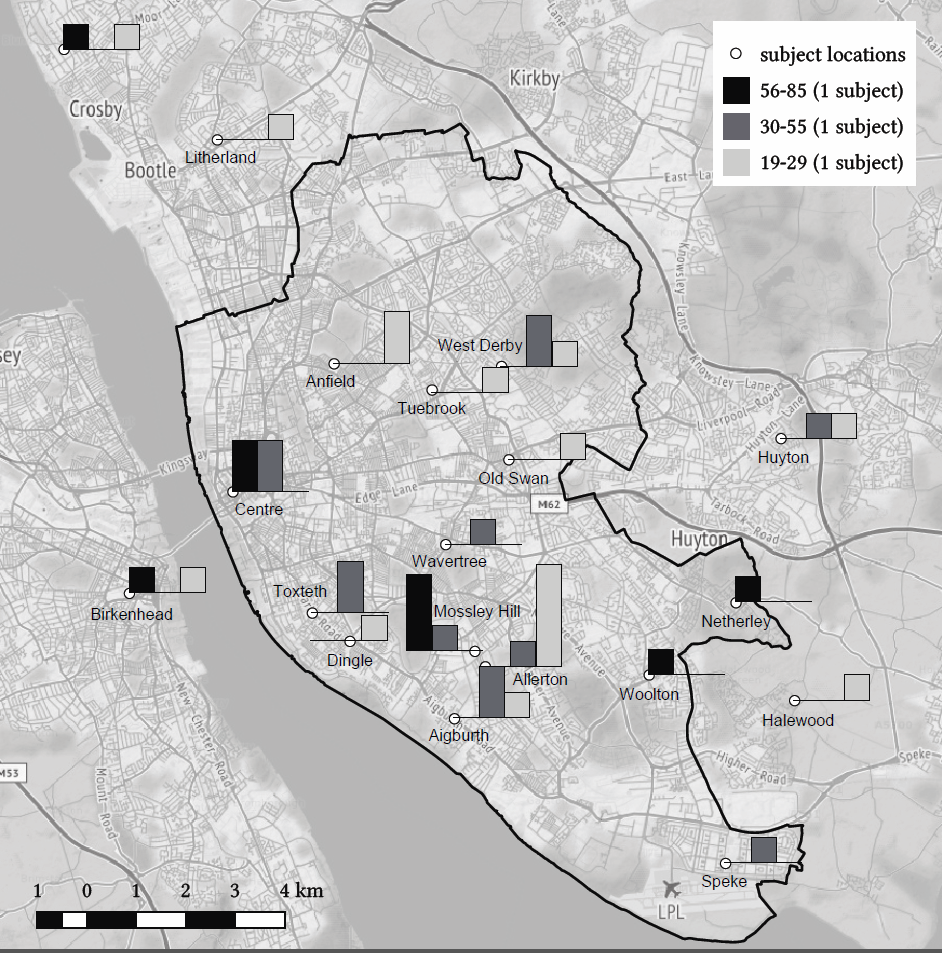
\includegraphics[width=0.8\textwidth]{figures/liverpool-participant-map.png}
		\caption{Geographical distribution of interview subjects}\label{fig.map.participants}
	\end{figure}

The study was not restricted to people from within the Liverpool Council boundaries (black line in the map), but also included areas which are administered by other local councils (Sefton, Knowsley, \isi{Wirral}) and which are, therefore, ``technically not Liverpool'' as a number of subjects put it. This is indeed, however, more of a technicality since we are talking about a contiguously built up area --- just like in most other urban agglomerations. It is clear that invisible lines (sometimes separating one side of a street from the other) can still be important for people's \isi{identity}, but all of the participants in this study self-identified as Liverpudlian\is{identity}s or Scouser\is{identity}s. This also held for the two subjects who were actually living on the \isi{Wirral} and who had both been born in Liverpool (and in one case also lived half her life within Liverpool city boundaries). Generally speaking, people in urban areas often move around quite a bit and this might be especially true for Liverpool where many people from inner city areas were actually relocated (sometimes very reluctantly so) to new housing estates on the outskirts of the city during the slum clearances of the 50s and 60s. This is indeed what many of the older participants experienced themselves. For these reasons it was deemed unjustified to restrict the pool of subjects to those living within Liverpool city boundaries only.

	\section{Transcription}\label{sec.prod_method.transcription}

All interviews were transcribed orthographically in Praat \parencite{praat} by the author.
Since the transcriptions' sole purpose was to serve as input for automatic measuring (cf. \ref{sec.prod_method.measuring}), pauses, \isi{intonation}, stress, etc. were not marked in the transcripts.
Questions and other utterances by the interviewer were equally ignored.
On separate tiers of the Praat TextGrid, speaking style (word ``list'', ``reading'' (passage), ``free'' (speech), and (accent) ``imitation\is{accent performance}'') and topic (``childhood'', ``Manchester'', ``\isi{identity}'' etc.) coded, followed by a third one where the participant's speech was segmented into chunks and transcribed.
Words containing test tokens and the individual variables themselves were marked on individual tiers called ``word'' and ``variable'' respectively.
Finally, a sixth tier called ``aspiration'' was used to mark relevant parts of the consonantal variables (cf. \ref{sec.prod_method.con}).
Figure \ref{fig.textgrid.ex} provides an extract from a TextGrid (zoomed to word level) for purposes of illustration.

	\begin{figure}[h]
		\centering
			\centering
			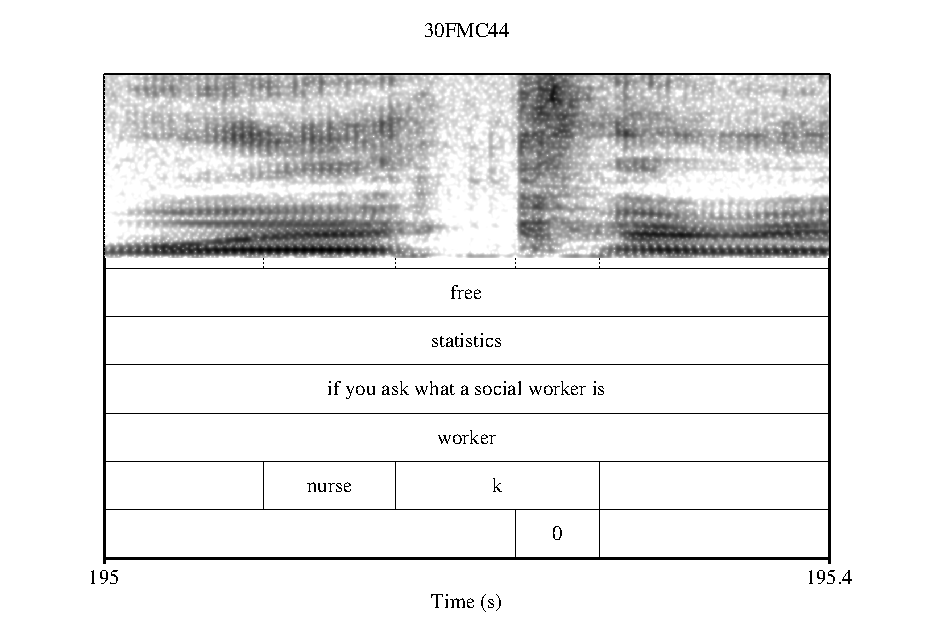
\includegraphics[width=0.75\textwidth]{figures/TextGrid_screenshot}
		\caption{Extract of Praat TextGrid (subject 30FMC44)}
		\label{fig.textgrid.ex}
	\end{figure}

	\section{Measuring}\label{sec.prod_method.measuring}

		\subsection{Consonants}\label{sec.prod_method.con}

The two consonantal variables were analysed both acoustically and auditorily.
The method for acoustic measuring of /k/ was heavily inspired by the one used in \citealt{sangster2001} to investigate lenition of alveolar stops. Phonetic plosives have a period of silence, or closure, followed by a burst and friction. For affricates, there is the same silence, but more friction than for plosives, and fricatives have either a very short period of silence or none at all and consist (almost) entirely of friction. 

Beginning and end of the friction phase were marked in a Praat TextGrid for every /k/. 
A script written by the author was then used to automatically measure the duration of these segments as well as the total durations of the plosives (i.e. including the closure phase).
/k/ tokens without any friction phase were registered as `unreleased' (and ignored in the analysis).
Next, what \citeauthor{sangster2001} calls `the proportional duration of friction' (\isi{PDF}) was calculated by dividing the duration of the friction phase by the total duration of the plosive. The result is a figure between 0 (or 0\%) and 1 (100\%), with lower values for more plosive-like realisations and higher values for sounds that are phonetically speaking affricates or fricatives.

The same technique was applied to /ŋ(g)/.
This decision might seem strange at first, because the realisational options of /ŋ(g)/ do not seem to be readily comparable to those of /k/.
Closer examination, however, reveals that the standard realisation as a nasal [ŋ] involves complete oral closure --- just as with [k] --- and that for the typical Scouse realisation as [ŋg] this closure phase is followed by a release burst / friction.
While the friction of [ŋg] will never be as long as that of a /k/ realised as a fricative, the \isi{PDF} values will mean the same thing for velar nasal plus as they do for /k/: lower values (no or little friction \(\rightarrow\) [ŋ]) indicate a standard-like realisation and higher scores (presence of friction \(\rightarrow\) [ŋg]) mark non-standard, Scouse variants.
Alveolar variants of /ŋ(g)/ were coded as ``in'' and later removed for the quantitative analyses for two reasons.
First, [n] is a non-standard variant that is not limited to Liverpool or even a clearly bounded region, but one that is used in all varieties of English English and many others as well.
It is also rather salient\is{salience} and commented on\is{overt commentary} by many non-linguists as \enquote*{g-dropping}.
However, in order to assess the impact of \isi{salience}, particularly in perception, this study required a local/regional feature with little or no \isi{salience}, to compare to the highly salient\is{salience} and local /k/ lenition.
Alveolar variants of the <ng> cluster fulfil neither criterion, while [ŋg] realisations tick both boxes.
The second reason concerns the method of measurement.
Realising <ng> as [n] by definition excludes the presence of even a hint of a plosive, so the \isi{PDF} measurement outlined above is not applicable.
The difference between [ŋ] and [ŋg] (or the devoiced\is{devoicing} variant [ŋk]), on the other hand, exhibits the same kind of gradualness and, as explained above, can be measured in the same way as /k/ lenition.
This parallelism is again crucial for the perception experiment, because it means the stimuli for /k/ and /ŋ(g)/ could be manipulated in a way that was phonetically similar (and thus not a confound).
Since linking up data from production and perception is a major interest of this study, the focus in the production part was also exclusively on the [ŋ]-[ŋg] distinction.
Figure \ref{fig.automatic.consonants} shows two examples and their respective marking in the TextGrid.

	\begin{figure}[h!]
		\centering
		\begin{subfigure}{0.75\textwidth}
			\centering
			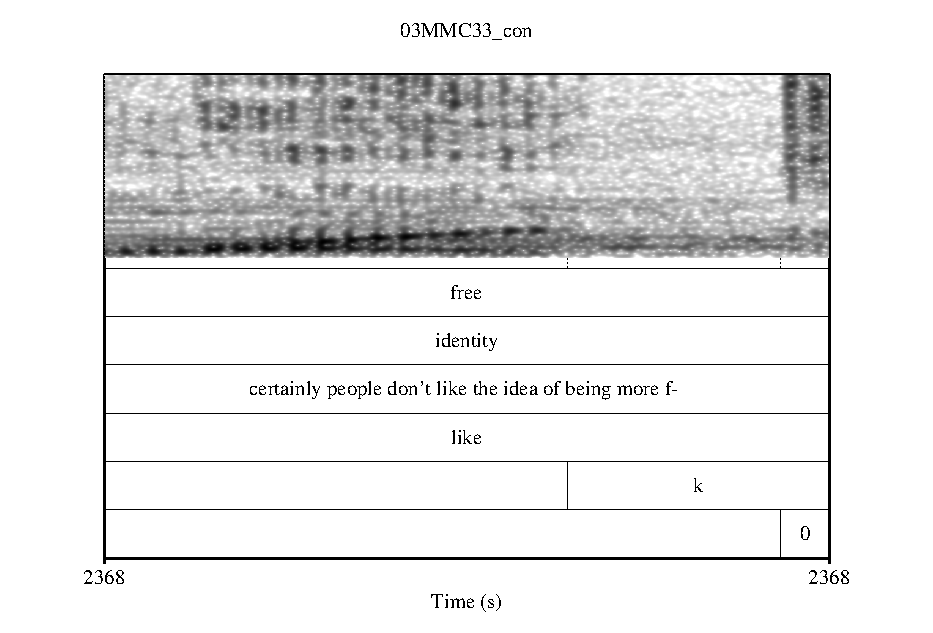
\includegraphics[width=\textwidth]{figures/like_plosive}
			\caption{plosive, PDF = 18.47\% (03MMC33)}
		\end{subfigure}
		\begin{subfigure}{0.75\textwidth}
			\centering
			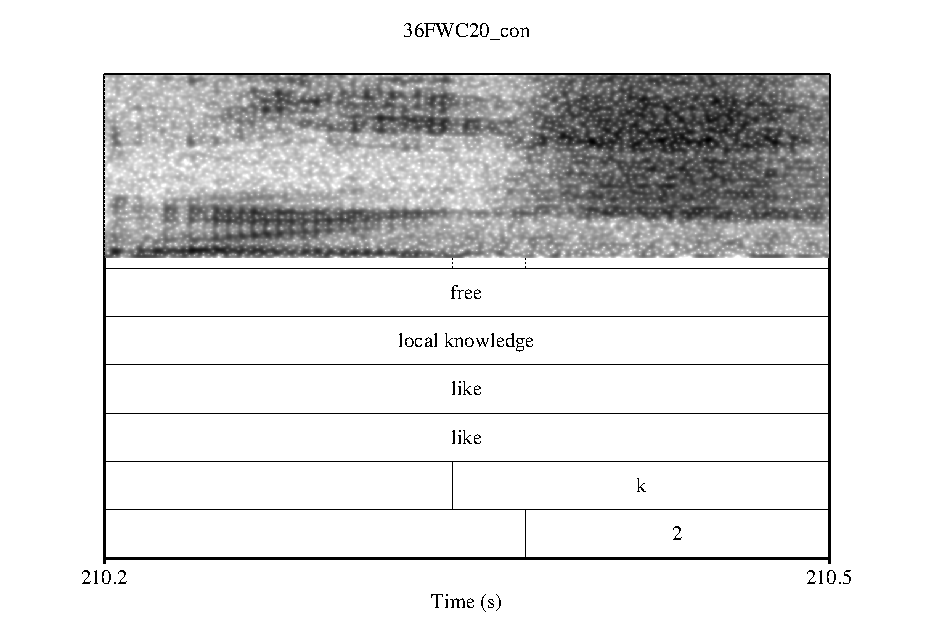
\includegraphics[width=\textwidth]{figures/like_fricative}
			\caption{fricative, PDF = 81.84\% (36FWC20)}
		\end{subfigure}
		\caption{Spectrograms of /k/ (zoomed to word level)}
		\label{fig.automatic.consonants}
	\end{figure}
	
This very precise method of acoustically measuring /k/ and velar nasal plus requires high quality recordings with little to no background noise.
As it was unclear at the beginning whether all interviews fulfilled these criteria, the data were also analysed auditorily by the author. 
Coding was `0' (plosive), `1' (affricate), and `2' (fricative) for /k/, and `0' (nasal) and `1' (nasal plus burst) for /ŋ(g)/.
It turned out that all interviews included in this project actually did permit an analysis based on the more precise \citeauthor{sangster2001} method, so the auditory coding was not used in the analysis in the end.
It is, however, still accessible for future research.

		\subsection{Vowels}\label{sec.prod_method.vow}
		
For the measurement of the first two (later three) vowel formants (\textsc{nurse}, \textsc{square}, and \textsc{happy}) a Praat script\footnote{generously made available by Mietta Lennes --- \url{http://www.helsinki.fi/~lennes/praat-scripts/}, last accessed 29/01/2013 --- and modified by the author} was used to automatise data collection.
\textsc{nurse} and \textsc{square} were measured first by hand and then in an automated way by the script for the first three (male) subjects.
Paired t-tests were then administered to make sure the automated measurements were reliable. Neither test ([t(545) = -0.975, p = 0.330] for F1 and [t(545) = 1.768, p = 0.078] for F2) found a significant difference between hand and automated measurements, although there was a trend for the F2 values.
However, the mean difference between hand and automated measurements for F2 was a mere 2.15 Hz.
Scatterplots furthermore show a near-perfect correlation of hand and automated measurements, which is why the script was deemed reliable and all formant measurements used in the final analysis were taken automatically only.
Clear mismeasurements were later removed from the dataset.

		\begin{figure}[h]
			\centering
				\begin{subfigure}[b]{0.45\textwidth}
					\centering
					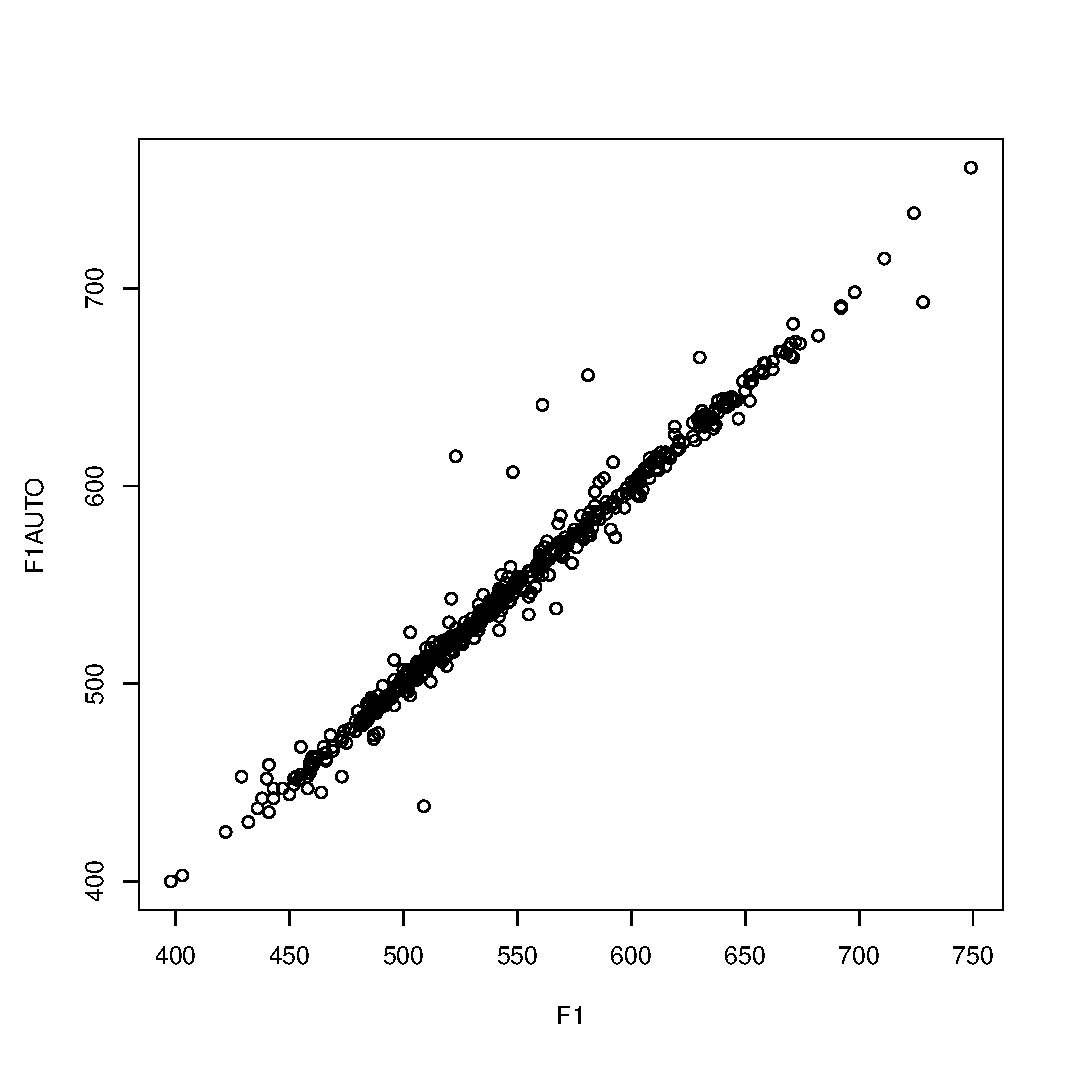
\includegraphics[width=\textwidth]{figures/F1F1AUTO}
					\caption{F1 measurements}
				\end{subfigure}
				\begin{subfigure}[b]{0.45\textwidth}
					\centering
					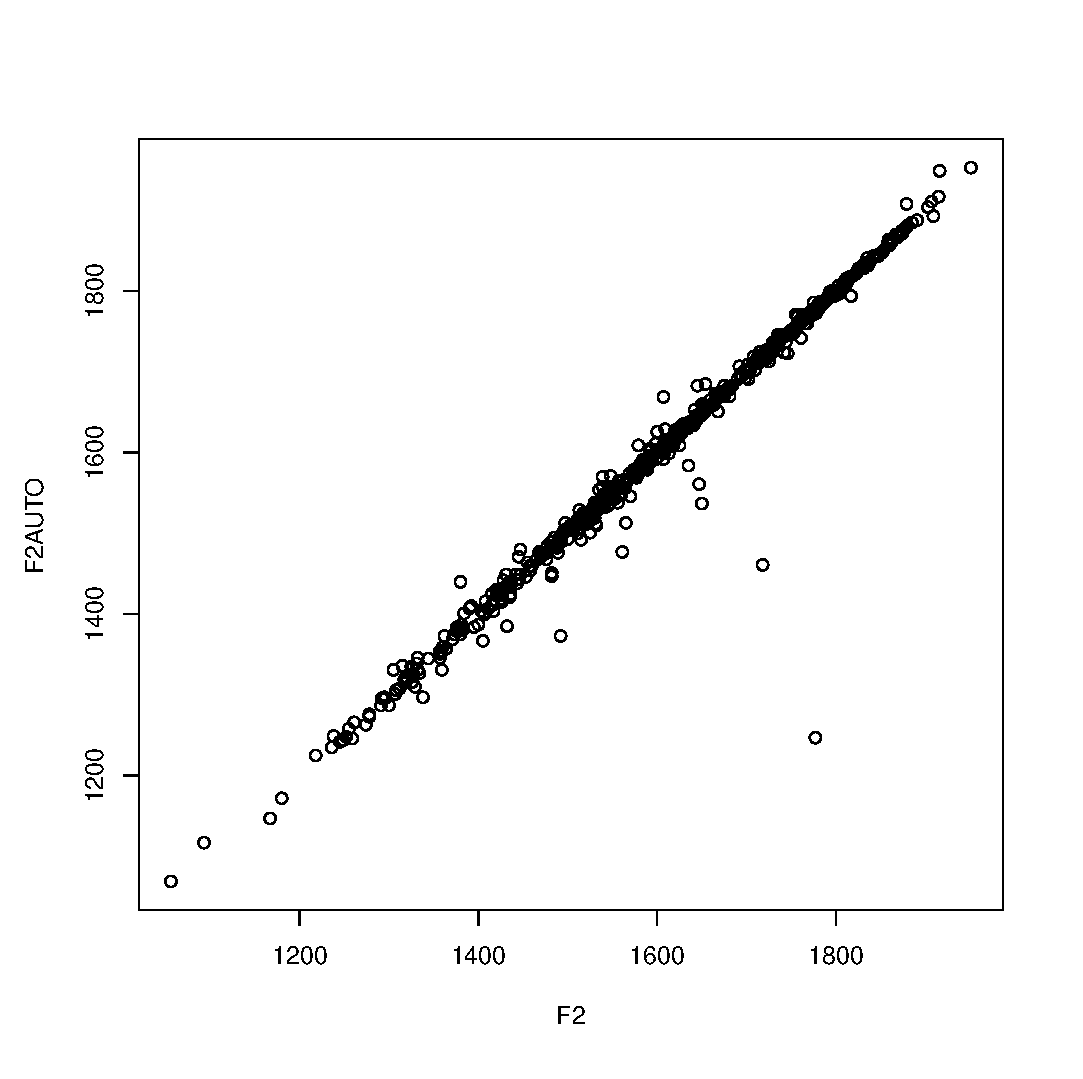
\includegraphics[width=\textwidth]{figures/F2F2AUTO}
					\caption{F2 measurements}
				\end{subfigure}
			\caption[Manual vs. automatic measurements (\textsc{nurse} and \textsc{square})]{Manual (x-axis) vs. automatic (y-axis) measurements of \textsc{nurse} and \textsc{square}}\label{fig.automatic.measurements}
		\end{figure}

The script took as input pairs of sound files and TextGrids.
It then went through each TextGrid and looked for vowel labels in the variable tier.
When it found a relevant label it noted the start and end of the segment and measured F1, F2, and F3 at midpoint of the vowel.
It then extracted information about the style, topic, carrier word, and the larger context it appeared in from the other tiers and saved all these data into a textfile.
F3 was measured because it was needed for one of the \isi{normalisation} algorithms that were later applied to the raw measurements (cf. \ref{sec.prod_method.norm}).
In addition to the three vocalic test variables happ\textsc{y}, \textsc{nurse}, and \textsc{square} (of which all instances were included), between 10 and 25 tokens of \textsc{fleece} and \textsc{trap} per subject were also measured.
These were taken from the reading passage and word list sections of the interviews since these contexts were considered most likely to produce the most `extreme' realisations (in terms of the periphery of speakers' vowel spaces).
Observations of \textsc{trap} were used exclusively as input for \isi{normalisation} and for comparison of the algorithms (again, cf. \ref{sec.prod_method.norm}).
\textsc{fleece} measurements were additionally included in the calculation of \isi{Pillai} scores for happ\textsc{y} (cf. \ref{sec.prod.res.vow.happy.pil}).

\subsection{Normalisation}\label{sec.prod_method.norm}

It is a well known fact among phoneticians and phonologists that there is a huge amount of variation in the acoustic signal that is not due to linguistic or sociolingustic, but rather purely physiological reasons.
Even multiple realisations of one and the same phonological sound chain produced by a single speaker in the same style will all be slightly different from one another.
In addition to these intra-speaker differences, there are also inter-speaker ones.
The most pronounced differences in this area are due to vocal tract length.
The length of the vocal tract correlates inversely with vowel formant values.
On average, therefore, children (with the shortest vocal tracts) have higher formants than women, who in turn have higher formants than men for one and the same phonological vowel.
The potential effect of vocal tract maturation, i.e. changes to length and shape of the vocal tract over the course of an individuals lifetime, further complicates matters \parencite[cf.][440--441]{harrington2006}.

It is therefore not possible (or at least not advisable) to directly compare, for instance, women's and men's raw formant values, or those of younger and older speakers.
This is where \isi{normalisation} comes in.
According to several articles on the matter \parencite[cf., for example,][]{fabriciusetal2009,clopper2009,disner1980,kendallthomas2014,thomas2002}, \isi{normalisation} should ideally achieve four different goals:
\begin{enumerate}
	\item \label{enum.norm.phys}elimination of differences that are due to physiological reasons
	\item \label{enum.norm.soc}preservation of differences that are (socio-)linguistic in nature
	\item \label{enum.norm.phon}preservation (or improvement) of phoneme distinctions
	\item \label{enum.norm.cog}modelling the process that allows listeners to assign realisations from different speakers to one and the same phoneme
\end{enumerate}
The author is well aware of the irony involved here.
This study is, after all, set in an \isi{exemplar} framework which suggests that listeners do \emph{not} normalise\is{normalisation} acoustic input, at least not in the same way and to the same degree as is assumed in most other phonological theories.
This is most relevant with respect to point \ref{enum.norm.cog} in the enumeration above. Sociolinguists, however, usually largely ignore this aspect and focus more on points \ref{enum.norm.phys} and \ref{enum.norm.soc} \parencites(cf.)()[1430]{clopper2009}[414--415]{fabriciusetal2009}{kendallthomas2014}, and the present study is no exception.
By applying a \isi{normalisation} algorithm to the data I do not mean to suggest that this procedure mirrors or approximates what happens in listeners' brains.
Rather, it is simply the only option one has if the goal is to compare production data of men and women (or those of younger and older speakers) to each other instead of treating them separately.

Normalisation methods are generally categorised with respect to two dimensions: vowel-intrinsic vs. vowel-extrinsic and speaker-intrinsic vs. speaker-extrinsic \parencite[cf.][]{kendallthomas2014}.
Vowel-intrinsic algorithms extract all data necessary for \isi{normalisation} from the individual token.
Often these methods use F0 and/or F3 to estimate vocal tract length.
Vowel-extrinsic algorithms include formant measurements from more than one vowel in their formulas and achieve \isi{normalisation} with the help of means over several (often all) measured vowels.
Speaker-intrinsic methods differ from speaker-extrinsic ones in that the former perform \isi{normalisation} for each speaker individually (i.e. only taking into account vowels produced by that speaker), whereas the latter include some sort of inter-speaker mean in their calculations (cf., for example, \textcite{labovetal2006}'s \emph{grand mean}).

A number of algorithms have been proposed over the years, and the question which of those fares best in achieving the goals spelled out above has generated a series of investigations \parencites(among others:)(){hindle1978}{disner1980}{adanketal2004}.
Generally speaking, ``vowel-extrinsic methods tend to perform better overall (\ldots) for vowel space normalization across talkers'', and ``vowel-intrinsic methods are appealing as perceptually plausible models of human speech processing'' \parencite[1440]{clopper2009}.
For this reason, two different \isi{normalisation} methods were tested in this study, a vowel-intrinsic and a vowel-extrinsic one (both of them speaker-intrinsic).
Both \isi{normalisation}s were applied to the raw data using the NORM package for R \parencite{kendallthomas2014}.
The first, Bark difference, was devised by \textcite{syrdalgopal1986}, and is a vowel-intrinsic method.
Formants are, first of all, transformed into --- perceptually ``more accurate'' \parencite[1431--1432]{clopper2009} --- Bark values using the formula taken from \textcite{traunmueller1990}:

\begin{equation}
	Z_{i} = \frac{26.81}{1 + \frac{1960}{F_{i}}} - 0.53
\end{equation}

Where \(F_{i}\) is the raw value of a given formant. The Bark rescaled values \(Z_{1}\) and \(Z_{2}\) are then substracted from \(Z_{3}\) to arrive at normalise\is{normalisation}d measures of height and frontness respectively. \citeauthor{syrdalgopal1986} originally used Bark-converted F0 instead of F3 for the height dimension, but \textcite{kendallthomas2014} argue that a number of things, for instance ``[i]ntonation, tone, and consonantal influences affect F0'' and consider it preferable to use Bark-converted F3 for both the back-front and the high-low dimension.

The most popular vowel-extrinsic \isi{normalisation} method among sociolinguists is probably \textcite{lobanov1971}.
This is unsurprising given the fact that it has frequently been found to be (one of) the most efficient algorithm(s) in reducing physiological and preserving sociolinguistic variation \parencite[cf.][1440]{clopper2009}.
The main drawback of \citeauthor{lobanov1971} --- and many other vowel-extrinsic algorithms --- is that it works best when \emph{all} vowels of a system are measured.
Constraints of time and resources made this endeavour impractical for the present study.
The choice fell on \textcite{wattfabricius2002} in its modified version \parencite{fabriciusetal2009} instead, a method which is ``conceptually similar'' and deemed ``also successful'' \parencite[1440]{clopper2009}.

\textcite{wattfabricius2002} assume a triangular vowel space with the `corner' vowels \([i]\), \([a]\), and \([u']\).
In RP (for which the algorithm was originally designed), these would correspond to \textsc{fleece}, \textsc{trap}, and \textsc{goose}, but
the NORM package automatically chooses the highest/most fronted and the most open vowel available in the sample as \([i]\) and \([a]\), irrespective of their labels.
Obviously, \([i]\) and \([a]\) should be relatively stable in the variety under scrutiny \parencite[cf.][163]{wattfabricius2002}.
Since I am not aware of any evidence that suggests this is \emph{not} true for \textsc{fleece} and \textsc{trap} in Scouse, these two were used as corners in this study.
From these benchmark vowels, a `centroid' S or ``centre of gravity'' \parencite[164]{wattfabricius2002} is then computed as follows:
\begin{equation}
	S(F_{n}) = \frac{[i]F_{n} + [a]F_{n} + [u']F_{n}}{3}
\end{equation}
Where \(F_{n}\) is a mean raw formant value of the corner vowels \([i]\), \([a]\), and \([u']\). The centroid value \(S(F_{n})\) is computed separately for each formant, and normalise\is{normalisation}d values are then expressed as the ratio of the raw measurement to the corresponding centroid: \(\frac{F_{n}}{S(F_{n})}\).
Note that \([u']\) is not measured, but derived from \([i]\), assuming that \([u']F_{1}\) = \([u']F_{2}\) = \([i]F_{1}\).
As a result, only \textsc{fleece} and \textsc{trap} have to be measured.
To counter potential skewing due to the fact that \textsc{trap} might not be exactly halfway between \textsc{fleece} and \textsc{goose} with respect to frontness, \([a]F_{2}\) is also derived instead of measured in the modified version of the algorithm employed in this study \parencites(cf.)()[420--421]{fabriciusetal2009}{kendallthomas2014}.

				\begin{figure}[h!]
					\centering
					\begin{subfigure}{.49\textwidth}
						\centering
						\resizebox{\linewidth}{!}{% Created by tikzDevice version 0.10.1 on 2017-03-15 16:22:39
% !TEX encoding = UTF-8 Unicode
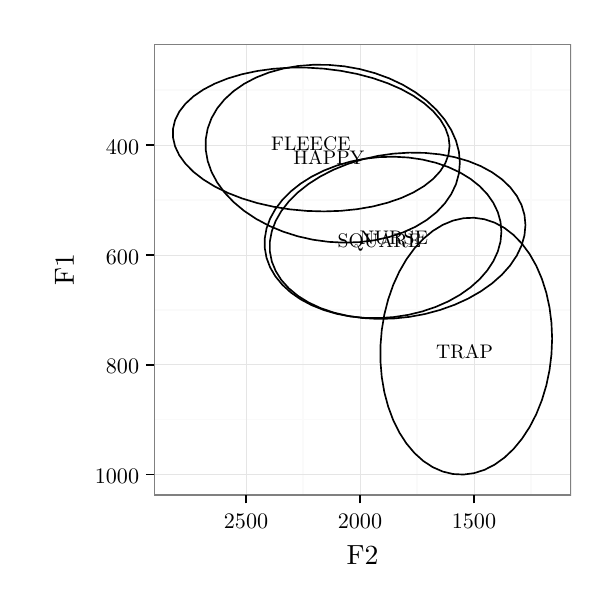
\begin{tikzpicture}[x=1pt,y=1pt]
\definecolor{fillColor}{RGB}{255,255,255}
\path[use as bounding box,fill=fillColor,fill opacity=0.00] (0,0) rectangle (202.36,202.36);
\begin{scope}
\path[clip] (  0.00,  0.00) rectangle (202.36,202.36);
\definecolor{drawColor}{RGB}{255,255,255}
\definecolor{fillColor}{RGB}{255,255,255}

\path[draw=drawColor,line width= 0.6pt,line join=round,line cap=round,fill=fillColor] (  0.00,  0.00) rectangle (202.36,202.36);
\end{scope}
\begin{scope}
\path[clip] ( 45.67, 33.48) rectangle (196.36,196.36);
\definecolor{fillColor}{RGB}{255,255,255}

\path[fill=fillColor] ( 45.67, 33.48) rectangle (196.36,196.36);
\definecolor{drawColor}{gray}{0.98}

\path[draw=drawColor,line width= 0.6pt,line join=round] ( 45.67,179.73) --
	(196.36,179.73);

\path[draw=drawColor,line width= 0.6pt,line join=round] ( 45.67,140.06) --
	(196.36,140.06);

\path[draw=drawColor,line width= 0.6pt,line join=round] ( 45.67,100.39) --
	(196.36,100.39);

\path[draw=drawColor,line width= 0.6pt,line join=round] ( 45.67, 60.72) --
	(196.36, 60.72);

\path[draw=drawColor,line width= 0.6pt,line join=round] (181.85, 33.48) --
	(181.85,196.36);

\path[draw=drawColor,line width= 0.6pt,line join=round] (140.67, 33.48) --
	(140.67,196.36);

\path[draw=drawColor,line width= 0.6pt,line join=round] ( 99.49, 33.48) --
	( 99.49,196.36);
\definecolor{drawColor}{gray}{0.90}

\path[draw=drawColor,line width= 0.2pt,line join=round] ( 45.67,159.89) --
	(196.36,159.89);

\path[draw=drawColor,line width= 0.2pt,line join=round] ( 45.67,120.22) --
	(196.36,120.22);

\path[draw=drawColor,line width= 0.2pt,line join=round] ( 45.67, 80.55) --
	(196.36, 80.55);

\path[draw=drawColor,line width= 0.2pt,line join=round] ( 45.67, 40.88) --
	(196.36, 40.88);

\path[draw=drawColor,line width= 0.2pt,line join=round] (161.26, 33.48) --
	(161.26,196.36);

\path[draw=drawColor,line width= 0.2pt,line join=round] (120.08, 33.48) --
	(120.08,196.36);

\path[draw=drawColor,line width= 0.2pt,line join=round] ( 78.90, 33.48) --
	( 78.90,196.36);
\definecolor{drawColor}{RGB}{0,0,0}

\node[text=drawColor,anchor=base,inner sep=0pt, outer sep=0pt, scale=  0.71] at (102.35,157.97) {FLEECE};

\node[text=drawColor,anchor=base,inner sep=0pt, outer sep=0pt, scale=  0.71] at (108.87,152.81) {HAPPY};

\node[text=drawColor,anchor=base,inner sep=0pt, outer sep=0pt, scale=  0.71] at (132.29,123.92) {NURSE};

\node[text=drawColor,anchor=base,inner sep=0pt, outer sep=0pt, scale=  0.71] at (127.12,123.10) {SQUARE};

\node[text=drawColor,anchor=base,inner sep=0pt, outer sep=0pt, scale=  0.71] at (157.86, 82.93) {TRAP};

\path[draw=drawColor,line width= 0.6pt,line join=round] (152.45,159.68) --
	(152.07,162.88) --
	(150.94,166.06) --
	(149.07,169.19) --
	(146.50,172.20) --
	(143.26,175.06) --
	(139.40,177.72) --
	(134.98,180.15) --
	(130.06,182.29) --
	(124.73,184.13) --
	(119.06,185.63) --
	(113.14,186.77) --
	(107.05,187.54) --
	(100.90,187.92) --
	( 94.76,187.91) --
	( 88.75,187.50) --
	( 82.94,186.70) --
	( 77.43,185.53) --
	( 72.30,184.01) --
	( 67.62,182.14) --
	( 63.47,179.98) --
	( 59.91,177.54) --
	( 57.00,174.86) --
	( 54.77,171.99) --
	( 53.27,168.96) --
	( 52.52,165.83) --
	( 52.52,162.64) --
	( 53.27,159.44) --
	( 54.77,156.28) --
	( 57.00,153.21) --
	( 59.91,150.26) --
	( 63.47,147.50) --
	( 67.62,144.95) --
	( 72.30,142.66) --
	( 77.43,140.67) --
	( 82.94,138.99) --
	( 88.75,137.67) --
	( 94.76,136.71) --
	(100.90,136.14) --
	(107.05,135.96) --
	(113.14,136.17) --
	(119.06,136.77) --
	(124.73,137.75) --
	(130.06,139.11) --
	(134.98,140.80) --
	(139.40,142.82) --
	(143.26,145.13) --
	(146.50,147.69) --
	(149.07,150.47) --
	(150.94,153.43) --
	(152.07,156.51) --
	(152.45,159.68);

\path[draw=drawColor,line width= 0.6pt,line join=round] (156.17,153.56) --
	(155.83,157.52) --
	(154.79,161.47) --
	(153.07,165.34) --
	(150.71,169.09) --
	(147.73,172.65) --
	(144.18,175.97) --
	(140.12,179.00) --
	(135.60,181.70) --
	(130.70,184.02) --
	(125.49,185.92) --
	(120.05,187.39) --
	(114.46,188.39) --
	(108.80,188.91) --
	(103.17,188.95) --
	( 97.64,188.50) --
	( 92.31,187.57) --
	( 87.24,186.18) --
	( 82.53,184.34) --
	( 78.23,182.08) --
	( 74.42,179.44) --
	( 71.15,176.46) --
	( 68.47,173.18) --
	( 66.43,169.65) --
	( 65.05,165.93) --
	( 64.35,162.07) --
	( 64.35,158.13) --
	( 65.05,154.17) --
	( 66.43,150.25) --
	( 68.47,146.44) --
	( 71.15,142.77) --
	( 74.42,139.33) --
	( 78.23,136.14) --
	( 82.53,133.28) --
	( 87.24,130.76) --
	( 92.31,128.65) --
	( 97.64,126.96) --
	(103.17,125.72) --
	(108.80,124.96) --
	(114.46,124.68) --
	(120.05,124.88) --
	(125.49,125.57) --
	(130.70,126.74) --
	(135.60,128.36) --
	(140.12,130.41) --
	(144.18,132.86) --
	(147.73,135.68) --
	(150.71,138.82) --
	(153.07,142.23) --
	(154.79,145.86) --
	(155.83,149.66) --
	(156.17,153.56);

\path[draw=drawColor,line width= 0.6pt,line join=round] (179.87,131.05) --
	(179.52,134.68) --
	(178.48,138.20) --
	(176.75,141.55) --
	(174.37,144.69) --
	(171.38,147.55) --
	(167.81,150.11) --
	(163.72,152.33) --
	(159.18,154.16) --
	(154.25,155.58) --
	(149.01,156.57) --
	(143.54,157.11) --
	(137.92,157.20) --
	(132.23,156.84) --
	(126.56,156.03) --
	(121.00,154.77) --
	(115.64,153.10) --
	(110.54,151.04) --
	(105.80,148.62) --
	(101.48,145.87) --
	( 97.64,142.83) --
	( 94.36,139.56) --
	( 91.66,136.10) --
	( 89.61,132.51) --
	( 88.22,128.83) --
	( 87.52,125.13) --
	( 87.52,121.46) --
	( 88.22,117.88) --
	( 89.61,114.44) --
	( 91.66,111.19) --
	( 94.36,108.18) --
	( 97.64,105.46) --
	(101.48,103.07) --
	(105.80,101.05) --
	(110.54, 99.42) --
	(115.64, 98.21) --
	(121.00, 97.44) --
	(126.56, 97.12) --
	(132.23, 97.26) --
	(137.92, 97.85) --
	(143.54, 98.88) --
	(149.01,100.35) --
	(154.25,102.22) --
	(159.18,104.46) --
	(163.72,107.06) --
	(167.81,109.95) --
	(171.38,113.11) --
	(174.37,116.48) --
	(176.75,120.02) --
	(178.48,123.66) --
	(179.52,127.35) --
	(179.87,131.05);

\path[draw=drawColor,line width= 0.6pt,line join=round] (171.18,128.67) --
	(170.86,132.23) --
	(169.89,135.70) --
	(168.29,139.03) --
	(166.09,142.18) --
	(163.32,145.09) --
	(160.01,147.72) --
	(156.23,150.03) --
	(152.03,151.98) --
	(147.46,153.55) --
	(142.61,154.71) --
	(137.54,155.44) --
	(132.34,155.73) --
	(127.07,155.58) --
	(121.83,155.00) --
	(116.68,153.98) --
	(111.71,152.54) --
	(106.99,150.71) --
	(102.60,148.52) --
	( 98.60,145.99) --
	( 95.05,143.17) --
	( 92.01,140.10) --
	( 89.51,136.82) --
	( 87.61,133.38) --
	( 86.32,129.85) --
	( 85.68,126.26) --
	( 85.68,122.68) --
	( 86.32,119.15) --
	( 87.61,115.74) --
	( 89.51,112.50) --
	( 92.01,109.46) --
	( 95.05,106.69) --
	( 98.60,104.21) --
	(102.60,102.08) --
	(106.99,100.32) --
	(111.71, 98.95) --
	(116.68, 98.00) --
	(121.83, 97.49) --
	(127.07, 97.42) --
	(132.34, 97.79) --
	(137.54, 98.59) --
	(142.61, 99.82) --
	(147.46,101.46) --
	(152.03,103.47) --
	(156.23,105.84) --
	(160.01,108.51) --
	(163.32,111.47) --
	(166.09,114.65) --
	(168.29,118.01) --
	(169.89,121.50) --
	(170.86,125.07) --
	(171.18,128.67);

\path[draw=drawColor,line width= 0.6pt,line join=round] (189.51, 90.01) --
	(189.27, 95.69) --
	(188.57,101.23) --
	(187.41,106.57) --
	(185.81,111.61) --
	(183.80,116.28) --
	(181.40,120.52) --
	(178.66,124.25) --
	(175.61,127.42) --
	(172.30,129.98) --
	(168.78,131.89) --
	(165.11,133.13) --
	(161.33,133.67) --
	(157.51,133.51) --
	(153.70,132.65) --
	(149.97,131.10) --
	(146.37,128.89) --
	(142.94,126.04) --
	(139.76,122.61) --
	(136.86,118.65) --
	(134.28,114.20) --
	(132.07,109.35) --
	(130.27,104.17) --
	(128.88, 98.73) --
	(127.95, 93.11) --
	(127.48, 87.41) --
	(127.48, 81.70) --
	(127.95, 76.08) --
	(128.88, 70.63) --
	(130.27, 65.43) --
	(132.07, 60.57) --
	(134.28, 56.10) --
	(136.86, 52.11) --
	(139.76, 48.66) --
	(142.94, 45.79) --
	(146.37, 43.55) --
	(149.97, 41.97) --
	(153.70, 41.07) --
	(157.51, 40.88) --
	(161.33, 41.39) --
	(165.11, 42.60) --
	(168.78, 44.49) --
	(172.30, 47.02) --
	(175.61, 50.16) --
	(178.66, 53.87) --
	(181.40, 58.08) --
	(183.80, 62.74) --
	(185.81, 67.77) --
	(187.41, 73.09) --
	(188.57, 78.63) --
	(189.27, 84.30) --
	(189.51, 90.01);
\definecolor{drawColor}{gray}{0.50}

\path[draw=drawColor,line width= 0.6pt,line join=round,line cap=round] ( 45.67, 33.48) rectangle (196.36,196.36);
\end{scope}
\begin{scope}
\path[clip] (  0.00,  0.00) rectangle (202.36,202.36);
\definecolor{drawColor}{RGB}{0,0,0}

\node[text=drawColor,anchor=base east,inner sep=0pt, outer sep=0pt, scale=  0.80] at ( 40.27,156.59) {400};

\node[text=drawColor,anchor=base east,inner sep=0pt, outer sep=0pt, scale=  0.80] at ( 40.27,116.92) {600};

\node[text=drawColor,anchor=base east,inner sep=0pt, outer sep=0pt, scale=  0.80] at ( 40.27, 77.25) {800};

\node[text=drawColor,anchor=base east,inner sep=0pt, outer sep=0pt, scale=  0.80] at ( 40.27, 37.58) {1000};
\end{scope}
\begin{scope}
\path[clip] (  0.00,  0.00) rectangle (202.36,202.36);
\definecolor{drawColor}{RGB}{0,0,0}

\path[draw=drawColor,line width= 0.6pt,line join=round] ( 42.67,159.89) --
	( 45.67,159.89);

\path[draw=drawColor,line width= 0.6pt,line join=round] ( 42.67,120.22) --
	( 45.67,120.22);

\path[draw=drawColor,line width= 0.6pt,line join=round] ( 42.67, 80.55) --
	( 45.67, 80.55);

\path[draw=drawColor,line width= 0.6pt,line join=round] ( 42.67, 40.88) --
	( 45.67, 40.88);
\end{scope}
\begin{scope}
\path[clip] (  0.00,  0.00) rectangle (202.36,202.36);
\definecolor{drawColor}{RGB}{0,0,0}

\path[draw=drawColor,line width= 0.6pt,line join=round] (161.26, 30.48) --
	(161.26, 33.48);

\path[draw=drawColor,line width= 0.6pt,line join=round] (120.08, 30.48) --
	(120.08, 33.48);

\path[draw=drawColor,line width= 0.6pt,line join=round] ( 78.90, 30.48) --
	( 78.90, 33.48);
\end{scope}
\begin{scope}
\path[clip] (  0.00,  0.00) rectangle (202.36,202.36);
\definecolor{drawColor}{RGB}{0,0,0}

\node[text=drawColor,anchor=base,inner sep=0pt, outer sep=0pt, scale=  0.80] at (161.26, 21.47) {1500};

\node[text=drawColor,anchor=base,inner sep=0pt, outer sep=0pt, scale=  0.80] at (120.08, 21.47) {2000};

\node[text=drawColor,anchor=base,inner sep=0pt, outer sep=0pt, scale=  0.80] at ( 78.90, 21.47) {2500};
\end{scope}
\begin{scope}
\path[clip] (  0.00,  0.00) rectangle (202.36,202.36);
\definecolor{drawColor}{RGB}{0,0,0}

\node[text=drawColor,anchor=base,inner sep=0pt, outer sep=0pt, scale=  1.00] at (121.01,  8.40) {F2};
\end{scope}
\begin{scope}
\path[clip] (  0.00,  0.00) rectangle (202.36,202.36);
\definecolor{drawColor}{RGB}{0,0,0}

\node[text=drawColor,rotate= 90.00,anchor=base,inner sep=0pt, outer sep=0pt, scale=  1.00] at ( 16.67,114.92) {F1};
\end{scope}
\end{tikzpicture}
}
						\caption{raw data}
						\label{fig.plot.scatter.raw}
					\end{subfigure}
					
					\begin{subfigure}{.49\textwidth}
						\centering
						\resizebox{\linewidth}{!}{% Created by tikzDevice version 0.10.1 on 2017-03-15 16:22:56
% !TEX encoding = UTF-8 Unicode
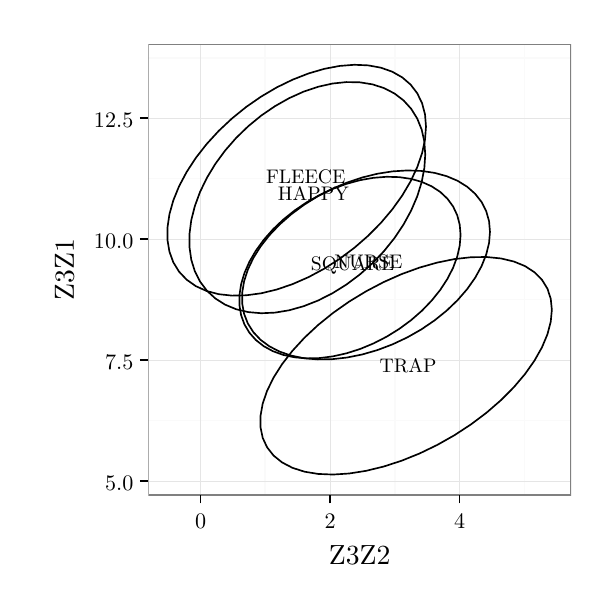
\begin{tikzpicture}[x=1pt,y=1pt]
\definecolor{fillColor}{RGB}{255,255,255}
\path[use as bounding box,fill=fillColor,fill opacity=0.00] (0,0) rectangle (202.36,202.36);
\begin{scope}
\path[clip] (  0.00,  0.00) rectangle (202.36,202.36);
\definecolor{drawColor}{RGB}{255,255,255}
\definecolor{fillColor}{RGB}{255,255,255}

\path[draw=drawColor,line width= 0.6pt,line join=round,line cap=round,fill=fillColor] (  0.00,  0.00) rectangle (202.36,202.36);
\end{scope}
\begin{scope}
\path[clip] ( 43.58, 33.48) rectangle (196.36,196.36);
\definecolor{fillColor}{RGB}{255,255,255}

\path[fill=fillColor] ( 43.58, 33.48) rectangle (196.36,196.36);
\definecolor{drawColor}{gray}{0.98}

\path[draw=drawColor,line width= 0.6pt,line join=round] ( 43.58, 60.42) --
	(196.36, 60.42);

\path[draw=drawColor,line width= 0.6pt,line join=round] ( 43.58,104.12) --
	(196.36,104.12);

\path[draw=drawColor,line width= 0.6pt,line join=round] ( 43.58,147.82) --
	(196.36,147.82);

\path[draw=drawColor,line width= 0.6pt,line join=round] ( 43.58,191.51) --
	(196.36,191.51);

\path[draw=drawColor,line width= 0.6pt,line join=round] ( 85.87, 33.48) --
	( 85.87,196.36);

\path[draw=drawColor,line width= 0.6pt,line join=round] (132.68, 33.48) --
	(132.68,196.36);

\path[draw=drawColor,line width= 0.6pt,line join=round] (179.49, 33.48) --
	(179.49,196.36);
\definecolor{drawColor}{gray}{0.90}

\path[draw=drawColor,line width= 0.2pt,line join=round] ( 43.58, 38.57) --
	(196.36, 38.57);

\path[draw=drawColor,line width= 0.2pt,line join=round] ( 43.58, 82.27) --
	(196.36, 82.27);

\path[draw=drawColor,line width= 0.2pt,line join=round] ( 43.58,125.97) --
	(196.36,125.97);

\path[draw=drawColor,line width= 0.2pt,line join=round] ( 43.58,169.67) --
	(196.36,169.67);

\path[draw=drawColor,line width= 0.2pt,line join=round] ( 62.47, 33.48) --
	( 62.47,196.36);

\path[draw=drawColor,line width= 0.2pt,line join=round] (109.28, 33.48) --
	(109.28,196.36);

\path[draw=drawColor,line width= 0.2pt,line join=round] (156.08, 33.48) --
	(156.08,196.36);
\definecolor{drawColor}{RGB}{0,0,0}

\node[text=drawColor,anchor=base,inner sep=0pt, outer sep=0pt, scale=  0.71] at (100.49,146.02) {FLEECE};

\node[text=drawColor,anchor=base,inner sep=0pt, outer sep=0pt, scale=  0.71] at (103.25,139.78) {HAPPY};

\node[text=drawColor,anchor=base,inner sep=0pt, outer sep=0pt, scale=  0.71] at (123.15,115.34) {NURSE};

\node[text=drawColor,anchor=base,inner sep=0pt, outer sep=0pt, scale=  0.71] at (117.45,114.60) {SQUARE};

\node[text=drawColor,anchor=base,inner sep=0pt, outer sep=0pt, scale=  0.71] at (137.43, 77.78) {TRAP};

\path[draw=drawColor,line width= 0.6pt,line join=round] (143.93,166.62) --
	(143.58,171.01) --
	(142.52,175.04) --
	(140.77,178.66) --
	(138.37,181.79) --
	(135.34,184.40) --
	(131.73,186.45) --
	(127.60,187.91) --
	(123.00,188.74) --
	(118.02,188.95) --
	(112.72,188.53) --
	(107.18,187.48) --
	(101.50,185.82) --
	( 95.74,183.57) --
	( 90.01,180.78) --
	( 84.39,177.47) --
	( 78.96,173.71) --
	( 73.81,169.54) --
	( 69.01,165.04) --
	( 64.64,160.27) --
	( 60.76,155.30) --
	( 57.44,150.21) --
	( 54.71,145.07) --
	( 52.63,139.96) --
	( 51.23,134.97) --
	( 50.52,130.16) --
	( 50.52,125.61) --
	( 51.23,121.39) --
	( 52.63,117.56) --
	( 54.71,114.18) --
	( 57.44,111.30) --
	( 60.76,108.96) --
	( 64.64,107.21) --
	( 69.01,106.06) --
	( 73.81,105.54) --
	( 78.96,105.65) --
	( 84.39,106.38) --
	( 90.01,107.74) --
	( 95.74,109.70) --
	(101.50,112.22) --
	(107.18,115.28) --
	(112.72,118.82) --
	(118.02,122.79) --
	(123.00,127.13) --
	(127.60,131.78) --
	(131.73,136.66) --
	(135.34,141.70) --
	(138.37,146.83) --
	(140.77,151.96) --
	(142.52,157.02) --
	(143.58,161.93) --
	(143.93,166.62);

\path[draw=drawColor,line width= 0.6pt,line join=round] (143.66,156.52) --
	(143.34,161.17) --
	(142.38,165.51) --
	(140.79,169.48) --
	(138.59,173.02) --
	(135.83,176.07) --
	(132.54,178.58) --
	(128.77,180.53) --
	(124.58,181.88) --
	(120.03,182.61) --
	(115.20,182.70) --
	(110.15,182.17) --
	(104.96,181.01) --
	( 99.71,179.24) --
	( 94.49,176.89) --
	( 89.36,173.99) --
	( 84.41,170.60) --
	( 79.71,166.75) --
	( 75.33,162.52) --
	( 71.35,157.96) --
	( 67.81,153.14) --
	( 64.78,148.13) --
	( 62.29,143.02) --
	( 60.40,137.87) --
	( 59.11,132.78) --
	( 58.47,127.80) --
	( 58.47,123.03) --
	( 59.11,118.52) --
	( 60.40,114.36) --
	( 62.29,110.60) --
	( 64.78,107.30) --
	( 67.81,104.51) --
	( 71.35,102.27) --
	( 75.33,100.62) --
	( 79.71, 99.58) --
	( 84.41, 99.17) --
	( 89.36, 99.39) --
	( 94.49,100.24) --
	( 99.71,101.71) --
	(104.96,103.77) --
	(110.15,106.40) --
	(115.20,109.55) --
	(120.03,113.18) --
	(124.58,117.22) --
	(128.77,121.63) --
	(132.54,126.33) --
	(135.83,131.25) --
	(138.59,136.32) --
	(140.79,141.46) --
	(142.38,146.59) --
	(143.34,151.64) --
	(143.66,156.52);

\path[draw=drawColor,line width= 0.6pt,line join=round] (167.05,128.59) --
	(166.72,132.43) --
	(165.70,136.03) --
	(164.03,139.34) --
	(161.72,142.30) --
	(158.82,144.87) --
	(155.36,147.02) --
	(151.40,148.70) --
	(147.00,149.90) --
	(142.22,150.59) --
	(137.14,150.77) --
	(131.83,150.43) --
	(126.38,149.58) --
	(120.86,148.22) --
	(115.37,146.39) --
	(109.98,144.11) --
	(104.78,141.41) --
	( 99.84,138.33) --
	( 95.24,134.92) --
	( 91.05,131.24) --
	( 87.33,127.34) --
	( 84.14,123.27) --
	( 81.53,119.10) --
	( 79.54,114.89) --
	( 78.20,110.71) --
	( 77.52,106.62) --
	( 77.52,102.68) --
	( 78.20, 98.96) --
	( 79.54, 95.50) --
	( 81.53, 92.35) --
	( 84.14, 89.58) --
	( 87.33, 87.22) --
	( 91.05, 85.30) --
	( 95.24, 83.86) --
	( 99.84, 82.91) --
	(104.78, 82.48) --
	(109.98, 82.56) --
	(115.37, 83.16) --
	(120.86, 84.26) --
	(126.38, 85.86) --
	(131.83, 87.92) --
	(137.14, 90.42) --
	(142.22, 93.31) --
	(147.00, 96.56) --
	(151.40,100.11) --
	(155.36,103.91) --
	(158.82,107.90) --
	(161.72,112.03) --
	(164.03,116.22) --
	(165.70,120.42) --
	(166.72,124.57) --
	(167.05,128.59);

\path[draw=drawColor,line width= 0.6pt,line join=round] (156.43,127.47) --
	(156.12,131.14) --
	(155.22,134.58) --
	(153.73,137.74) --
	(151.67,140.56) --
	(149.08,143.00) --
	(145.99,145.02) --
	(142.46,146.61) --
	(138.53,147.72) --
	(134.26,148.35) --
	(129.73,148.48) --
	(124.99,148.11) --
	(120.13,147.26) --
	(115.21,145.92) --
	(110.31,144.12) --
	(105.50,141.90) --
	(100.85,139.27) --
	( 96.45,136.29) --
	( 92.34,133.00) --
	( 88.60,129.44) --
	( 85.29,125.67) --
	( 82.44,121.76) --
	( 80.11,117.75) --
	( 78.33,113.71) --
	( 77.13,109.69) --
	( 76.53,105.77) --
	( 76.53,102.00) --
	( 77.13, 98.44) --
	( 78.33, 95.13) --
	( 80.11, 92.14) --
	( 82.44, 89.51) --
	( 85.29, 87.27) --
	( 88.60, 85.46) --
	( 92.34, 84.11) --
	( 96.45, 83.24) --
	(100.85, 82.86) --
	(105.50, 82.97) --
	(110.31, 83.59) --
	(115.21, 84.69) --
	(120.13, 86.25) --
	(124.99, 88.27) --
	(129.73, 90.70) --
	(134.26, 93.51) --
	(138.53, 96.65) --
	(142.46,100.08) --
	(145.99,103.75) --
	(149.08,107.60) --
	(151.67,111.57) --
	(153.73,115.61) --
	(155.22,119.64) --
	(156.12,123.61) --
	(156.43,127.47);

\path[draw=drawColor,line width= 0.6pt,line join=round] (189.41,100.42) --
	(189.01,104.41) --
	(187.82,108.04) --
	(185.85,111.24) --
	(183.14,113.97) --
	(179.73,116.20) --
	(175.66,117.87) --
	(171.00,118.97) --
	(165.83,119.49) --
	(160.21,119.41) --
	(154.24,118.74) --
	(148.00,117.48) --
	(141.59,115.66) --
	(135.10,113.30) --
	(128.64,110.43) --
	(122.31,107.11) --
	(116.19,103.39) --
	(110.38, 99.31) --
	(104.97, 94.94) --
	(100.05, 90.35) --
	( 95.68, 85.60) --
	( 91.93, 80.77) --
	( 88.86, 75.93) --
	( 86.52, 71.16) --
	( 84.93, 66.53) --
	( 84.14, 62.10) --
	( 84.14, 57.95) --
	( 84.93, 54.13) --
	( 86.52, 50.71) --
	( 88.86, 47.74) --
	( 91.93, 45.26) --
	( 95.68, 43.31) --
	(100.05, 41.91) --
	(104.97, 41.10) --
	(110.38, 40.88) --
	(116.19, 41.26) --
	(122.31, 42.23) --
	(128.64, 43.77) --
	(135.10, 45.87) --
	(141.59, 48.48) --
	(148.00, 51.58) --
	(154.24, 55.11) --
	(160.21, 59.02) --
	(165.83, 63.25) --
	(171.00, 67.74) --
	(175.66, 72.42) --
	(179.73, 77.22) --
	(183.14, 82.06) --
	(185.85, 86.87) --
	(187.82, 91.58) --
	(189.01, 96.12) --
	(189.41,100.42);
\definecolor{drawColor}{gray}{0.50}

\path[draw=drawColor,line width= 0.6pt,line join=round,line cap=round] ( 43.58, 33.48) rectangle (196.36,196.36);
\end{scope}
\begin{scope}
\path[clip] (  0.00,  0.00) rectangle (202.36,202.36);
\definecolor{drawColor}{RGB}{0,0,0}

\node[text=drawColor,anchor=base east,inner sep=0pt, outer sep=0pt, scale=  0.80] at ( 38.18, 35.26) {5.0};

\node[text=drawColor,anchor=base east,inner sep=0pt, outer sep=0pt, scale=  0.80] at ( 38.18, 78.96) {7.5};

\node[text=drawColor,anchor=base east,inner sep=0pt, outer sep=0pt, scale=  0.80] at ( 38.18,122.66) {10.0};

\node[text=drawColor,anchor=base east,inner sep=0pt, outer sep=0pt, scale=  0.80] at ( 38.18,166.36) {12.5};
\end{scope}
\begin{scope}
\path[clip] (  0.00,  0.00) rectangle (202.36,202.36);
\definecolor{drawColor}{RGB}{0,0,0}

\path[draw=drawColor,line width= 0.6pt,line join=round] ( 40.58, 38.57) --
	( 43.58, 38.57);

\path[draw=drawColor,line width= 0.6pt,line join=round] ( 40.58, 82.27) --
	( 43.58, 82.27);

\path[draw=drawColor,line width= 0.6pt,line join=round] ( 40.58,125.97) --
	( 43.58,125.97);

\path[draw=drawColor,line width= 0.6pt,line join=round] ( 40.58,169.67) --
	( 43.58,169.67);
\end{scope}
\begin{scope}
\path[clip] (  0.00,  0.00) rectangle (202.36,202.36);
\definecolor{drawColor}{RGB}{0,0,0}

\path[draw=drawColor,line width= 0.6pt,line join=round] ( 62.47, 30.48) --
	( 62.47, 33.48);

\path[draw=drawColor,line width= 0.6pt,line join=round] (109.28, 30.48) --
	(109.28, 33.48);

\path[draw=drawColor,line width= 0.6pt,line join=round] (156.08, 30.48) --
	(156.08, 33.48);
\end{scope}
\begin{scope}
\path[clip] (  0.00,  0.00) rectangle (202.36,202.36);
\definecolor{drawColor}{RGB}{0,0,0}

\node[text=drawColor,anchor=base,inner sep=0pt, outer sep=0pt, scale=  0.80] at ( 62.47, 21.47) {0};

\node[text=drawColor,anchor=base,inner sep=0pt, outer sep=0pt, scale=  0.80] at (109.28, 21.47) {2};

\node[text=drawColor,anchor=base,inner sep=0pt, outer sep=0pt, scale=  0.80] at (156.08, 21.47) {4};
\end{scope}
\begin{scope}
\path[clip] (  0.00,  0.00) rectangle (202.36,202.36);
\definecolor{drawColor}{RGB}{0,0,0}

\node[text=drawColor,anchor=base,inner sep=0pt, outer sep=0pt, scale=  1.00] at (119.97,  8.40) {Z3Z2};
\end{scope}
\begin{scope}
\path[clip] (  0.00,  0.00) rectangle (202.36,202.36);
\definecolor{drawColor}{RGB}{0,0,0}

\node[text=drawColor,rotate= 90.00,anchor=base,inner sep=0pt, outer sep=0pt, scale=  1.00] at ( 16.67,114.92) {Z3Z1};
\end{scope}
\end{tikzpicture}
}
						\caption{Bark difference normalised}
						\label{fig.plot.scatter.bark}
					\end{subfigure}
					\begin{subfigure}{.49\textwidth}
						\centering
						\resizebox{\linewidth}{!}{% Created by tikzDevice version 0.10.1 on 2017-03-15 16:22:58
% !TEX encoding = UTF-8 Unicode
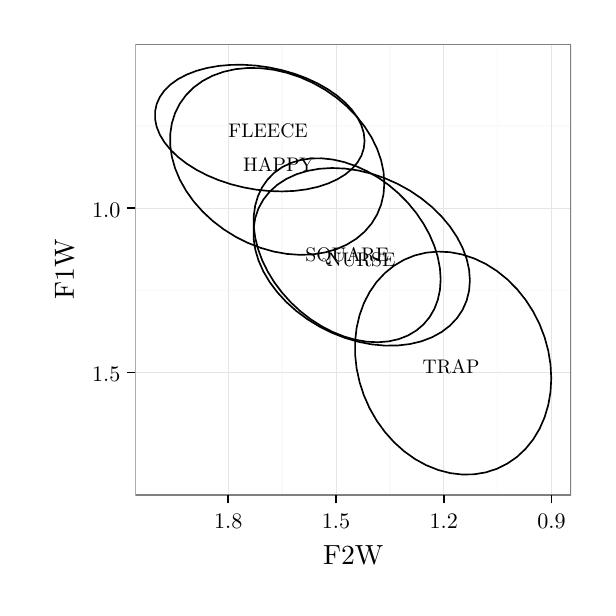
\begin{tikzpicture}[x=1pt,y=1pt]
\definecolor{fillColor}{RGB}{255,255,255}
\path[use as bounding box,fill=fillColor,fill opacity=0.00] (0,0) rectangle (202.36,202.36);
\begin{scope}
\path[clip] (  0.00,  0.00) rectangle (202.36,202.36);
\definecolor{drawColor}{RGB}{255,255,255}
\definecolor{fillColor}{RGB}{255,255,255}

\path[draw=drawColor,line width= 0.6pt,line join=round,line cap=round,fill=fillColor] (  0.00,  0.00) rectangle (202.36,202.36);
\end{scope}
\begin{scope}
\path[clip] ( 38.88, 33.48) rectangle (196.36,196.36);
\definecolor{fillColor}{RGB}{255,255,255}

\path[fill=fillColor] ( 38.88, 33.48) rectangle (196.36,196.36);
\definecolor{drawColor}{gray}{0.98}

\path[draw=drawColor,line width= 0.6pt,line join=round] ( 38.88,166.79) --
	(196.36,166.79);

\path[draw=drawColor,line width= 0.6pt,line join=round] ( 38.88,107.43) --
	(196.36,107.43);

\path[draw=drawColor,line width= 0.6pt,line join=round] (169.81, 33.48) --
	(169.81,196.36);

\path[draw=drawColor,line width= 0.6pt,line join=round] (130.89, 33.48) --
	(130.89,196.36);

\path[draw=drawColor,line width= 0.6pt,line join=round] ( 91.97, 33.48) --
	( 91.97,196.36);
\definecolor{drawColor}{gray}{0.90}

\path[draw=drawColor,line width= 0.2pt,line join=round] ( 38.88,137.11) --
	(196.36,137.11);

\path[draw=drawColor,line width= 0.2pt,line join=round] ( 38.88, 77.75) --
	(196.36, 77.75);

\path[draw=drawColor,line width= 0.2pt,line join=round] (189.27, 33.48) --
	(189.27,196.36);

\path[draw=drawColor,line width= 0.2pt,line join=round] (150.35, 33.48) --
	(150.35,196.36);

\path[draw=drawColor,line width= 0.2pt,line join=round] (111.43, 33.48) --
	(111.43,196.36);

\path[draw=drawColor,line width= 0.2pt,line join=round] ( 72.50, 33.48) --
	( 72.50,196.36);
\definecolor{drawColor}{RGB}{0,0,0}

\node[text=drawColor,anchor=base,inner sep=0pt, outer sep=0pt, scale=  0.71] at ( 86.89,162.51) {FLEECE};

\node[text=drawColor,anchor=base,inner sep=0pt, outer sep=0pt, scale=  0.71] at ( 90.71,150.28) {HAPPY};

\node[text=drawColor,anchor=base,inner sep=0pt, outer sep=0pt, scale=  0.71] at (120.57,116.10) {NURSE};

\node[text=drawColor,anchor=base,inner sep=0pt, outer sep=0pt, scale=  0.71] at (115.47,117.90) {SQUARE};

\node[text=drawColor,anchor=base,inner sep=0pt, outer sep=0pt, scale=  0.71] at (153.00, 77.50) {TRAP};

\path[draw=drawColor,line width= 0.6pt,line join=round] (121.74,161.44) --
	(121.45,164.23) --
	(120.60,167.05) --
	(119.18,169.85) --
	(117.23,172.60) --
	(114.78,175.25) --
	(111.85,177.76) --
	(108.50,180.09) --
	(104.78,182.21) --
	(100.74,184.09) --
	( 96.44,185.69) --
	( 91.96,186.99) --
	( 87.35,187.98) --
	( 82.69,188.64) --
	( 78.04,188.95) --
	( 73.48,188.92) --
	( 69.08,188.54) --
	( 64.91,187.82) --
	( 61.02,186.77) --
	( 57.48,185.41) --
	( 54.33,183.75) --
	( 51.64,181.83) --
	( 49.43,179.67) --
	( 47.75,177.30) --
	( 46.61,174.76) --
	( 46.04,172.09) --
	( 46.04,169.33) --
	( 46.61,166.52) --
	( 47.75,163.70) --
	( 49.43,160.92) --
	( 51.64,158.22) --
	( 54.33,155.63) --
	( 57.48,153.21) --
	( 61.02,150.98) --
	( 64.91,148.98) --
	( 69.08,147.23) --
	( 73.48,145.78) --
	( 78.04,144.63) --
	( 82.69,143.80) --
	( 87.35,143.32) --
	( 91.96,143.18) --
	( 96.44,143.38) --
	(100.74,143.93) --
	(104.78,144.82) --
	(108.50,146.03) --
	(111.85,147.54) --
	(114.78,149.33) --
	(117.23,151.38) --
	(119.18,153.65) --
	(120.60,156.11) --
	(121.45,158.72) --
	(121.74,161.44);

\path[draw=drawColor,line width= 0.6pt,line join=round] (128.88,146.19) --
	(128.59,150.29) --
	(127.71,154.44) --
	(126.27,158.59) --
	(124.28,162.67) --
	(121.77,166.62) --
	(118.78,170.38) --
	(115.35,173.89) --
	(111.55,177.10) --
	(107.42,179.96) --
	(103.03,182.42) --
	( 98.45,184.46) --
	( 93.73,186.04) --
	( 88.97,187.13) --
	( 84.22,187.72) --
	( 79.57,187.80) --
	( 75.07,187.36) --
	( 70.80,186.42) --
	( 66.83,185.00) --
	( 63.21,183.10) --
	( 59.99,180.76) --
	( 57.24,178.02) --
	( 54.98,174.91) --
	( 53.26,171.49) --
	( 52.10,167.80) --
	( 51.51,163.90) --
	( 51.51,159.86) --
	( 52.10,155.72) --
	( 53.26,151.56) --
	( 54.98,147.44) --
	( 57.24,143.42) --
	( 59.99,139.56) --
	( 63.21,135.92) --
	( 66.83,132.55) --
	( 70.80,129.51) --
	( 75.07,126.84) --
	( 79.57,124.59) --
	( 84.22,122.78) --
	( 88.97,121.44) --
	( 93.73,120.60) --
	( 98.45,120.26) --
	(103.03,120.44) --
	(107.42,121.13) --
	(111.55,122.31) --
	(115.35,123.98) --
	(118.78,126.10) --
	(121.77,128.65) --
	(124.28,131.58) --
	(126.27,134.85) --
	(127.71,138.41) --
	(128.59,142.21) --
	(128.88,146.19);

\path[draw=drawColor,line width= 0.6pt,line join=round] (159.80,111.03) --
	(159.50,114.90) --
	(158.62,118.84) --
	(157.16,122.79) --
	(155.14,126.70) --
	(152.61,130.49) --
	(149.59,134.11) --
	(146.13,137.52) --
	(142.29,140.65) --
	(138.12,143.47) --
	(133.68,145.92) --
	(129.05,147.97) --
	(124.29,149.59) --
	(119.48,150.75) --
	(114.68,151.44) --
	(109.97,151.65) --
	(105.43,151.37) --
	(101.12,150.61) --
	( 97.11,149.38) --
	( 93.45,147.69) --
	( 90.20,145.58) --
	( 87.42,143.07) --
	( 85.14,140.21) --
	( 83.40,137.03) --
	( 82.23,133.59) --
	( 81.64,129.93) --
	( 81.64,126.12) --
	( 82.23,122.21) --
	( 83.40,118.26) --
	( 85.14,114.32) --
	( 87.42,110.47) --
	( 90.20,106.75) --
	( 93.45,103.23) --
	( 97.11, 99.95) --
	(101.12, 96.98) --
	(105.43, 94.34) --
	(109.97, 92.08) --
	(114.68, 90.25) --
	(119.48, 88.85) --
	(124.29, 87.92) --
	(129.05, 87.47) --
	(133.68, 87.51) --
	(138.12, 88.03) --
	(142.29, 89.03) --
	(146.13, 90.49) --
	(149.59, 92.39) --
	(152.61, 94.71) --
	(155.14, 97.40) --
	(157.16,100.42) --
	(158.62,103.74) --
	(159.50,107.29) --
	(159.80,111.03);

\path[draw=drawColor,line width= 0.6pt,line join=round] (149.23,111.39) --
	(148.97,115.35) --
	(148.21,119.41) --
	(146.95,123.50) --
	(145.21,127.57) --
	(143.02,131.55) --
	(140.41,135.39) --
	(137.42,139.03) --
	(134.10,142.40) --
	(130.50,145.47) --
	(126.67,148.18) --
	(122.66,150.49) --
	(118.55,152.37) --
	(114.39,153.78) --
	(110.25,154.72) --
	(106.19,155.15) --
	(102.26,155.09) --
	( 98.54,154.52) --
	( 95.07,153.46) --
	( 91.91,151.92) --
	( 89.10,149.92) --
	( 86.70,147.50) --
	( 84.73,144.69) --
	( 83.23,141.54) --
	( 82.21,138.09) --
	( 81.70,134.40) --
	( 81.70,130.52) --
	( 82.21,126.50) --
	( 83.23,122.42) --
	( 84.73,118.33) --
	( 86.70,114.30) --
	( 89.10,110.38) --
	( 91.91,106.63) --
	( 95.07,103.12) --
	( 98.54, 99.89) --
	(102.26, 97.00) --
	(106.19, 94.49) --
	(110.25, 92.39) --
	(114.39, 90.74) --
	(118.55, 89.56) --
	(122.66, 88.87) --
	(126.67, 88.69) --
	(130.50, 89.01) --
	(134.10, 89.82) --
	(137.42, 91.13) --
	(140.41, 92.90) --
	(143.02, 95.11) --
	(145.21, 97.73) --
	(146.95,100.71) --
	(148.21,104.02) --
	(148.97,107.60) --
	(149.23,111.39);

\path[draw=drawColor,line width= 0.6pt,line join=round] (189.20, 75.65) --
	(188.93, 80.60) --
	(188.13, 85.56) --
	(186.80, 90.45) --
	(184.98, 95.20) --
	(182.68, 99.74) --
	(179.94,103.99) --
	(176.81,107.90) --
	(173.32,111.40) --
	(169.54,114.45) --
	(165.52,116.99) --
	(161.32,118.98) --
	(157.00,120.41) --
	(152.64,121.23) --
	(148.29,121.45) --
	(144.02,121.06) --
	(139.90,120.07) --
	(135.99,118.48) --
	(132.35,116.33) --
	(129.04,113.65) --
	(126.09,110.47) --
	(123.57,106.85) --
	(121.50,102.84) --
	(119.93, 98.50) --
	(118.86, 93.89) --
	(118.32, 89.10) --
	(118.32, 84.18) --
	(118.86, 79.22) --
	(119.93, 74.29) --
	(121.50, 69.46) --
	(123.57, 64.80) --
	(126.09, 60.40) --
	(129.04, 56.31) --
	(132.35, 52.60) --
	(135.99, 49.32) --
	(139.90, 46.52) --
	(144.02, 44.25) --
	(148.29, 42.54) --
	(152.64, 41.41) --
	(157.00, 40.88) --
	(161.32, 40.97) --
	(165.52, 41.66) --
	(169.54, 42.96) --
	(173.32, 44.83) --
	(176.81, 47.25) --
	(179.94, 50.19) --
	(182.68, 53.59) --
	(184.98, 57.42) --
	(186.80, 61.60) --
	(188.13, 66.08) --
	(188.93, 70.79) --
	(189.20, 75.65);
\definecolor{drawColor}{gray}{0.50}

\path[draw=drawColor,line width= 0.6pt,line join=round,line cap=round] ( 38.88, 33.48) rectangle (196.36,196.36);
\end{scope}
\begin{scope}
\path[clip] (  0.00,  0.00) rectangle (202.36,202.36);
\definecolor{drawColor}{RGB}{0,0,0}

\node[text=drawColor,anchor=base east,inner sep=0pt, outer sep=0pt, scale=  0.80] at ( 33.48,133.80) {1.0};

\node[text=drawColor,anchor=base east,inner sep=0pt, outer sep=0pt, scale=  0.80] at ( 33.48, 74.44) {1.5};
\end{scope}
\begin{scope}
\path[clip] (  0.00,  0.00) rectangle (202.36,202.36);
\definecolor{drawColor}{RGB}{0,0,0}

\path[draw=drawColor,line width= 0.6pt,line join=round] ( 35.88,137.11) --
	( 38.88,137.11);

\path[draw=drawColor,line width= 0.6pt,line join=round] ( 35.88, 77.75) --
	( 38.88, 77.75);
\end{scope}
\begin{scope}
\path[clip] (  0.00,  0.00) rectangle (202.36,202.36);
\definecolor{drawColor}{RGB}{0,0,0}

\path[draw=drawColor,line width= 0.6pt,line join=round] (189.27, 30.48) --
	(189.27, 33.48);

\path[draw=drawColor,line width= 0.6pt,line join=round] (150.35, 30.48) --
	(150.35, 33.48);

\path[draw=drawColor,line width= 0.6pt,line join=round] (111.43, 30.48) --
	(111.43, 33.48);

\path[draw=drawColor,line width= 0.6pt,line join=round] ( 72.50, 30.48) --
	( 72.50, 33.48);
\end{scope}
\begin{scope}
\path[clip] (  0.00,  0.00) rectangle (202.36,202.36);
\definecolor{drawColor}{RGB}{0,0,0}

\node[text=drawColor,anchor=base,inner sep=0pt, outer sep=0pt, scale=  0.80] at (189.27, 21.47) {0.9};

\node[text=drawColor,anchor=base,inner sep=0pt, outer sep=0pt, scale=  0.80] at (150.35, 21.47) {1.2};

\node[text=drawColor,anchor=base,inner sep=0pt, outer sep=0pt, scale=  0.80] at (111.43, 21.47) {1.5};

\node[text=drawColor,anchor=base,inner sep=0pt, outer sep=0pt, scale=  0.80] at ( 72.50, 21.47) {1.8};
\end{scope}
\begin{scope}
\path[clip] (  0.00,  0.00) rectangle (202.36,202.36);
\definecolor{drawColor}{RGB}{0,0,0}

\node[text=drawColor,anchor=base,inner sep=0pt, outer sep=0pt, scale=  1.00] at (117.62,  8.40) {F2W};
\end{scope}
\begin{scope}
\path[clip] (  0.00,  0.00) rectangle (202.36,202.36);
\definecolor{drawColor}{RGB}{0,0,0}

\node[text=drawColor,rotate= 90.00,anchor=base,inner sep=0pt, outer sep=0pt, scale=  1.00] at ( 16.67,114.92) {F1W};
\end{scope}
\end{tikzpicture}
}
						\caption{Watt-Fabricius normalised}
						\label{fig.plot.scatter.watt}
					\end{subfigure}
					
					\caption{Vowel distributions (all subjects pooled)}
					\label{fig.normcomp}
				\end{figure}

With respect to the tests applied to assess the power of the \isi{normalisation} algorithms, this study largely follows \citealt{langstrofdiss}.
One criterion for determining whether a \isi{normalisation} process was successful is the degree to which it has reduced variance \emph{within} categories and overlap \emph{across} categories.
In our case this would mean that phonemes should be more distinct\is{distinctness} and that scatter around phoneme means should be reduced in the normalise\is{normalisation}d data.
When we look at Figure \ref{fig.plot.scatter.bark} this is not immediately obvious.
It should be borne in mind that with respect to \textsc{nurse} and \textsc{square} we are talking about a merger for most speakers so we would not necessarily expect these two phonemes to appear more distinct\is{distinctness} in normalise\is{normalisation}d data.
The third vowel under scrutiny here, happ\textsc{y}, however, should be more distant from both \textsc{nurse} and \textsc{square} in the normalise\is{normalisation}d data.
At least for the Bark-difference method, the graph does not suggest that it really is.

It does not look as if scatter for any of the variables had been reduced either.
If anything, scatter around the mean seems to have increased, particularly in the front-back dimension.
The scatter plot for the \citeauthor{wattfabricius2002} normalise\is{normalisation}d data looks a lot more promising.
Scatter in both dimensions seems to have been (slightly) reduced, and the phonemes appear to be more distinct\is{distinctness}.
But then again, we are using different scales in the three representations so a purely visual inspection is insufficient.
We will thus have a look at variation coefficients next.
I am well aware of the fact that the measure of dispersion most commonly used in such cases is the standard deviation. Since we have very different means in our samples due to different scales, however, comparing standard deviations would be highly misleading as they depend on the means of the samples. We will therefore use variation coefficients which normalise\is{normalisation} standard deviations by dividing them by the mean of the sample. These variation coefficients can then be meaningfully compared to each other.

\begin{table}[h]
	\centering
	\caption{Variation coefficients for raw and normalised data}
	\begin{tabular}{lllllll}
		\hline
		& \multicolumn{3}{c}{F1} & \multicolumn{3}{c}{F2}\\
		vowel & raw & Bark & Watt & raw & Bark & Watt\\
		\hline
		happ\textsc{y} &
		0.187 & 0.107 & 0.167 &
		0.120 & 0.506 & 0.089\\
		\textsc{nurse} &
		0.127 & 0.101 & 0.115 &
		0.139 & 0.356 & 0.104\\
		\textsc{square} &
		0.123 & 0.101 & 0.115 &
		0.123 & 0.363 & 0.084\\
		\hline
	\end{tabular}
	\label{tab.varcoeff}
\end{table}

Table \ref{tab.varcoeff} shows a rather mixed picture. While the Bark difference algorithm was successful in reducing variance in the F1 dimension for all three vowels, it actually \emph{increased} variance of F2 considerably for all vowels involved. We thus cannot clearly claim that the Bark difference \isi{normalisation} reduced within-vowel variance overall.
\citeauthor{wattfabricius2002} fares a lot better.
Reduction in variance for F1 is systematic, if only marginal and slightly less successful than Bark-difference.
When we look at F2, however, we see a clear improvement.
Again, the reduction in variance is not huge, but \citeauthor{wattfabricius2002} does reduce variance systematically across all three vowels, whereas Bark-difference actually \emph{in}creases variance dramatically.
On the whole, then, \citeauthor{wattfabricius2002} seems to do a better job than Bark-difference in reducing intra-category variance.

Next, we look at \isi{Pillai} scores as a measure of distance between distributions, in our case of vowel discreteness.
\isi{Pillai} scores were first used in a linguistic study by \textcite{hayetal2006b} and their usefulness for sociolinguistic investigations is discussed in \citealt{halllew2010}.
They are considered to be superior to simple Euclidean distance measures because a \isi{Pillai} score ``takes account of the degree of overlap of the entire distribution'' \parencite[467]{hayetal2006b}.
\isi{Pillai} scores range between 0 and 1, with values close to 0 (and an accompanying high p-value) indicating a large degree of overlap between the distributions, and values near 1 (and a low p-value) representing distributions that are (almost) completely distinct\is{distinctness}.
The pairing \textsc{nurse-square} is not represented in Table \ref{tab.pillai} as these two vowels participate in a merger for most speakers and it can therefore not be assumed that they \emph{should} be distinct\is{distinctness} in the first place.

\begin{table}[h]
	\centering
	\caption{Pillai scores for total and female/male vowel distributions}
	%\scriptsize
	\begin{tabular}{lllllll}
		\hline
		& \multicolumn{2}{c}{raw} & \multicolumn{2}{c}{Bark} & \multicolumn{2}{c}{Watt}\\
		vowel(s) & \isi{Pillai} & p-value & \isi{Pillai} & p-value & \isi{Pillai} & p-value\\
		\hline
		happ\textsc{y}-\textsc{nurse} &
		0.486 &
		< 0.001 &
		0.460 &
		< 0.001 &
		0.550 &
		< 0.001\\
		happ\textsc{y}-\textsc{square} &
		0.372 &
		< 0.001 &
		0.323 &
		< 0.001 &
		0.425 &
		< 0.001 \\
		happ\textsc{y} (female/male) &
		0.446 &
		< 0.001 &
		0.090 &
		< 0.001 &
		0.020 &
		< 0.001 \\
		\textsc{nurse} (female/male) &
		0.570 &
		< 0.001 &
		0.229 &
		< 0.001 &
		0.131 &
		< 0.001 \\
		\textsc{square} (female/male) &
		0.659 &
		< 0.001 &
		0.185 &
		< 0.001 &
		0.115 &
		< 0.001 \\
		\hline
	\end{tabular}
	\label{tab.pillai}
\end{table}

Table \ref{tab.pillai} confirms the impression we already got from Figure \ref{fig.normcomp}: the Bark difference \isi{normalisation} does not distinguish happ\textsc{y} from both \textsc{nurse} and \textsc{square} better.
We also see, however, that it does not really fare worse.
\isi{Pillai} scores for raw and normalise\is{normalisation}d data are very similar and p-values are close to 0 in both cases.
So while the Bark difference \isi{normalisation} did not make different phonemes appear more distinct\is{distinctness}, it did at least not result in significantly \emph{less} distinct\is{distinctness} categories either.
\citeauthor{wattfabricius2002}, on the other hand, increases the distinct\is{distinctness}ness of happ\textsc{y} to both \textsc{nurse} and \textsc{square}.
Only slightly so for the former, it has to be said, but quite clearly for the latter.
As is obvious from the table, p-values are extremely low for all pairings (often too small to be treated as different from zero by the R software), which is in all likelihood simply due to the fact that they are based on comparatively large datasets where even small differences will show up as (highly) significant.
When we look at the three vowels individually and compare female to male realisations, we see a clear `improvement' in the normalise\is{normalisation}d data.
For all three vowels, female and male realisations are quite distinct\is{distinctness} in the raw data, a fact which is reflected in \isi{Pillai} scores which are comparable or actually higher than those for different phonemes, and p-values that indicate highly significant differences. 

All \isi{Pillai} scores for the Bark difference normalise\is{normalisation}d data are lower than their counterparts calculated for the raw data.
Intra-category overlap has increased by 0.356 for happ\textsc{y}, 0.34 for \textsc{nurse}, and 0.474 for \textsc{square}.
This means that female vowels are more similar to male vowels in the normalise\is{normalisation}d data, which is precisely what we would expect a vowel \isi{normalisation} process to achieve.
Female and male distributions are still significantly different from each other in the normalise\is{normalisation}d data, but,
\begin{inparaenum}[(a)]
	\item again, this could simply be due to the fact that we have a comparatively large data set where even small differences will come out as significant (cf. the very low \isi{Pillai} score of 0.09 for happ\textsc{y}), and, more importantly,
	\item we do not want \emph{all} differences to be filtered out, but only the \emph{physiological} ones.
\end{inparaenum}

All three vowels are test vowels in this study and we expect to see at least some gender differences which are due to sociolinguistic rather than physiological reasons.
This is particularly true for the \textsc{nurse-square} merger, a sociolinguistic variable which is considered to be highly salient\is{salience} (cf. Chapter \ref{ch.var}) and with respect to which we would therefore not be surprised to see women and men behave differently.
happ\textsc{y}, on the other hand, is believed to be non-salient\is{salience} (again, cf. Chapter \ref{ch.var}), so gender differences are less likely here.
This is exactly what the figures in Table \ref{tab.pillai} suggest: a very low \isi{Pillai} score for happ\textsc{y}, indicating almost complete overlap of the distributions (although this small difference is still significant) and considerably larger ones for \textsc{nurse} and \textsc{square}, meaning that women and men differ in their realisations of these vowels even \emph{after} \isi{normalisation}.
It thus appears as if the Bark difference \isi{normalisation} had (largely) eliminated physiological variation but maintained sociolinguistic one, which is just what we want a useful \isi{normalisation} procedure to do.

The values for our other candidate, however, are even better.
\citeauthor{wattfabricius2002} increases intra-category overlap for happ\textsc{y} by 0.426, for \textsc{nurse} by 0.439, and for \textsc{square} by 0.545.
The remaining differences between female/male distributions are also less (though still highly) significant in the \citeauthor{wattfabricius2002} normalise\is{normalisation}d data.
It is possible that \citeauthor{wattfabricius2002} has in fact eliminated some information that we are interested in, namely the assumed sociolinguistic gender difference for \textsc{nurse} and \textsc{square}.
However, the figures show that although the gender distributions are less distinct\is{distinctness} than in the Bark-difference normalise\is{normalisation}d data, they are still (and by a much larger factor than in the Bark values) more distinct\is{distinctness} than the normalise\is{normalisation}d female/male distributions of happ\textsc{y}.
Also, it could very well be that the smaller differences we find for \textsc{nurse} and \textsc{square} in the \citeauthor{wattfabricius2002} normalise\is{normalisation}d data are simply the more realistic ones.
Both algorithms thus create a pronounced relative difference between the female/male \isi{Pillai} scores of happ\textsc{y} and those of \textsc{nurse} and \textsc{square}, but in addition \citeauthor{wattfabricius2002} decreases inter-phoneme overlap more, so the conclusion with respect to \isi{Pillai} scores is again that \citeauthor{wattfabricius2002} seems to be the preferable choice.

Euclidean distance measures can also be used to determine the usefulness of \isi{normalisation} procedures. Once again, we cannot directly compare euclidean distances because of different scales. What we can do, however is look at a ratio that is calculated as follows:

\begin{equation}
	\frac{d_{k}}{d_{l}} = \frac{\langle\sqrt{(F_{1i} - \bar{F_{1j}})^2 + (F_{2i} - \bar{F_{2j}})^2}\rangle}
	{\langle\sqrt{(F_{1i} - \bar{F_{1i}})^2 + (F_{2i} - \bar{F_{2i}})^2}\rangle}
\end{equation}

Where \(F_{1i}\) and \(F_{2i}\) are the F1 and F2 values of tokens in phoneme category `i', \(\bar{F_{1i}}\) and \(\bar{F_{2i}}\) are the mean values of category `i', and \(\bar{F_{1j}}\) and \(\bar{F_{2j}}\) are the mean values of category `j'. \(d_{k}\) is then the average distance of tokens in category `i' to the mean of category `j' (e.g. happ\textsc{y} tokens to the mean of \textsc{nurse}), and \(d_{l}\) is the average distance of tokens in category `i' to their own mean (e.g. happ\textsc{y} tokens to the mean of happ\textsc{y}). This ratio should always be greater than 1, i.e. the average distance to the mean of \emph{another} category should be bigger than the average distance to the mean \emph{within} the category. A successful \isi{normalisation} procedure would have to increase this ratio since both intra-category spread and inter-category overlap should be diminished.

\begin{table}[h]
	\centering
	\caption{Euclidean distance ratios for raw and normalised data}
	\begin{tabular}{llll}
		\hline
		vowels & raw & Bark & Watt\\
		\hline
		happ\textsc{y}-\textsc{nurse} &
		1.574 &
		1.599 &
		2.326 \\
		happ\textsc{y}-\textsc{square} &
		1.429 &
		1.533 &
		2.187 \\
		\textsc{nurse}-happ\textsc{y} &
		1.694 &
		1.741 &
		2.320 \\
		\textsc{square}-happ\textsc{y} &
		1.579 &
		1.786 &
		2.355 \\
		\hline
	\end{tabular}
	\label{tab.euclid}
\end{table}

Table \ref{tab.euclid} shows that, while the difference is marginal for the pairing happ\textsc{y}-\textsc{nurse}, all euclidean distance ratios are higher for the Bark difference normalise\is{normalisation}d data than for the raw data.
Normalisation using this method was therefore an improvement.
Yet the figures for \citeauthor{wattfabricius2002} are, once again, even better.
While the distance ratio increases on average only by about 0.096 for the Bark-difference normalise\is{normalisation}d data, \citeauthor{wattfabricius2002} produces distance ratios that are on average 0.728 higher.

With the current dataset \citeauthor{wattfabricius2002} thus yields better results than the Bark-difference method in visual representation (scatter plots), reduction of inter-category variation coefficients, \isi{Pillai} scores for inter- and intra-category (gender) comparisons, and euclidean distance ratios.
Despite the fact that the Bark-difference \isi{normalisation} is presumably more plausible in perceptual terms, the \citeauthor{wattfabricius2002} algorithm will therefore be used in this study whenever normalise\is{normalisation}d vowel values or plots are reported or represented.

\section{Phonological context}
\label{sec.prod_method.phon}

In order to extract the \isi{phonological context} of the variables under scrutiny orthographical representations of the carrier word and the one following the carrier word were extracted from the transcripts.
These orthographic representations were then automatically replaced (in R) by a phonemic transcription that was gathered from the interactive web-based CELEX lexicon database \parencite{baayenetal1993}.
With regard to those transcriptions, CELEX allows the user to choose from four different character sets.
For this study, the DISC set was selected because it represents each English phoneme with a single character (vowel length is not coded separately as this bit of information is already included in the vowel quality --- in English!).
This is highly useful if the transcriptions are going to be processed automatically, as diphthongs and affricates (which are regarded as single phonemes) are represented by a single character.
It is therefore impossible to misinterpret the first element of a diphthong (or and affricate) as a simple monophthong (or plosive).
This is a crucial advantage, as the software often has no straightforward way of knowing whether it is faced with a diphthong or a sequence of monophthongs.
DISC uses a set of simple ASCII characters.
In Table \ref{tab.DISC} the characters that are different from IPA are listed together with their IPA equivalents.

	\begin{table}[h]
		\centering
		\caption{DISC characters and IPA equivalents}
		\begin{tabular}{cccccc}
			\hline
			\multicolumn{2}{c}{consonants} & \multicolumn{2}{c}{monophthongs} & \multicolumn{2}{c}{diphthongs}\\
			IPA & DISC & IPA & DISC & IPA & DISC\\
			\hline
			ŋ & N & ɪ & I & eɪ & 1\\
			θ & T & ɛ & E & aɪ & 2\\
			ð & D & æ & \{ & ɔɪ & 4\\
			ʃ & S & ʌ & V & əʊ & 5\\
			ʒ & Z & ɒ & Q & ɑʊ & 6\\
			t͡ʃ & J & ʊ & U & ɪə & 7\\
			d͡ʒ & \_ & ə & @ & ɛə & 8\\
			ŋ̩ & C & iː & i & ʊə & 9\\
			m̩̩ & F & ɑː & \# &&\\
			n̩ & H & ɔː & \$ &&\\
			l̩ & P & ɜː & 3 &&\\
			\hline
		\end{tabular}
		\label{tab.DISC}
	\end{table}

The impact of neighbouring sounds on the test variables \emph{will} be investigated to provide a more complete picture of how these sounds are used in Liverpool.
However, since the focus of this study is clearly on independent variables that are social in nature, this part of the analysis will be rather basic.
Only the immediately preceding and the immediately following phonemes are considered.
In the case of the two consonantal variables, measurements were furthermore restricted, from the start, to cases where /ŋ(g)/ and /k/ occurred either intervocallically or at the end of a word, because these contexts have been identified as the ones where lenition is most likely to occur (cf. \ref{sec.var.con.len}).
The three test vowels were only measured in content words (and, for \textsc{nurse} and \textsc{square}, also exclusively in stressed syllables), both to keep the number of vowels that had to be measured manageable and in order to avoid introducing unnecessary noise into the dataset by including weakened vowels.

All but two measured vowels either occurred at the beginning of a stretch of speech or were preceded by a consonant.
\textsc{nurse} and \textsc{square} tokens, without exception, either were the last phoneme in a stretch of speech or were \emph{followed} by a consonant, too.
Only happ\textsc{y} had a sizeable proportion of observations where the test vowel was followed by another vowel.
The difference between happ\textsc{y} measurements followed by a consonant and those followed by a vowel was small but significiant with respect to the normalise\is{normalisation}d F1 dimension (t(2016.295) = -13.593, p < 0.001), but insignificant as far as the (sociolinguistically more important, \citealt[cf.][502]{labov2006a}) F2 dimension is concerned (t(1935.124) = -1.355, p = 0.176).
It was therefore decided to drop happ\textsc{y} tokens that occurred before another vowel (along with \emph{any} observation where a test vowel was followed or preceded by silence) when fitting mixed linear effects regression models (see \ref{sec.prod_method.stats}) because this allowed me to use the same set of phonological predictors (place and manner of preceding and following consonant) for all three vocalic test variables and thereby improved comparability of the models.
Measurements of happ\textsc{y} still accounted for the largest share of total observations, and in figures and other statistical comparisons (t-tests), the complete data set (including happ\textsc{y} followed by another vowel) was used.
Of course, this meant that it could not be investigated whether happ\textsc{y} formants might be influenced by vowel harmony.
This is an interesting question, but given the focus of the present analysis, it was considered outside of the scope of this thesis anyway, and will have to be addressed in a separate study in the future.
Word frequencies were considered for all variables investigated, and operationalised using Zipf\is{Zipf score} scores based on occurrences in SUBTLEX-UK \parencite{heuvenetal2014}.
See \ref{sec.perc_method.sentences} for a more detailed discussion.

	\section{Statistical analysis}
	\label{sec.prod_method.stats}

Mixed linear effects models have become a sort of gold standard in recent years, especially in subdisciplines like psycho- and neurolinguistics.
Their biggest advantage is the possibility to include so-called random effects.
The reasoning behind this is that in most common experimental designs, we have ``fixed effects'' and ``random effects''.
Fixed effects are the variables the experimenter is primarily interested in and which are, as a consequence, controlled for in the experiment.
They are theorised to have the same or a similar impact in the sample that is the basis for the experiment as in the total population which the sample is drawn from.
Random effects, on the other hand, are responsible for variation that is not part of the experimental design, but due to the particular sample.
As a result, the effects of random factors cannot be extrapolated to the population as a whole \parencite[cf.][]{barretal2013}.

In Mixed linear effects models, the impact of random factors is estimated and taken out of the data before the relevance of the fixed effects is calculated.
The result is a reduction in noise since variation that is supposed to be due to chance is filtered out.
As a common example, consider a hypothetical lexical decision experiment where subjects have to decide whether a particular string of sounds or letters is a word of their language.
The words that are presented fall into two intrinsically different groups (e.g. different word class, length, complexity,\ldots) and the experimenter is interested in whether reaction times for these two word groups differ.
In such an example it is often found that individual words produce generally higher or lower reaction times across subjects (e.g. due to a non-controlled factor such as \isi{frequency} or number of similar words in the language).
The experimenter, however, is not interested in the effect of particular words but only in the general effect of the group they are part of.
The actual words chosen for the experiment are, in this case, considered a random sample of the whole group (\(\rightarrow\) population).
The same goes for the sample of participants, as some people are generally faster or slower to respond than other subjects.
Both sources of variation are `random' because re-running the experiment would (or at least \emph{could}) involve choosing a different sample of words and a different sample of participants \parencite[cf.][259--260]{barretal2013}.
It thus makes sense to filter out variation that is due to individual differences between subjects and test words as it is a characteristic of the sample, and not considered representative of the population.

It was thoroughly considered whether subject and carrier word --- the two most straightforward options --- should be entered as random factors in an analysis of the production data presented here.
Especially with respect to word, this would make some sense.
After all, there is no control over which words subjects use the relevant variables in (at least in the free speech part of the interviews which makes up the vast majority of observations).
Treating carrier word as a random factor was still deemed problematic, however.
This is because the \isi{frequency} of the carrier word, as well as the sounds directly preceding and following the target sound are factors of theoretical interest here.
While word itself could be considered a random factor in this research design, it seems likely that filtering out word effects would also eliminate a lot of \emph{relevant} information that is coded in the variables `preceding sound', `following sound', and `word \isi{frequency}', as these bits of information (among others) are included in the overall word context of the observation.
In the end, the risk was considered worth taking in order to counteract a scenario where (highly frequent) individual words would otherwise unjustifiably dominate the sample, and --- possibly --- obscure or overlay any more general effects of \isi{frequency} or phonological environment\is{phonological context}.

Treating interviewee as a random effect is even more of an issue.
As explained above, the reasoning behind treating subject as a random effect in many psycho-linguistic experiments is that the group of people that actually took part is a random subset of the population one wants to extrapolate the results to and that individual differences are therefore noise.
This crucial assumption, however, is not met in the dataset that is analysed in this chapter.
There was no active a priori selection of participants (cf. \ref{sec.prod_method.participants}) in terms of typicality etc.
Nonetheless, the participants that ended up in the sample \emph{are} considered to be representative of their social group.
We look at a comparatively small number of middle- and working-class (female/male, old/young\ldots) speakers and analyse their speech because we believe our results \emph{can} be generalised to the group as a whole (at least to a certain extent).
This is an essential tenet of any sociolinguistic analysis and argues against treating participant as a random effect.

It is possible to calculate random effects for speaker sub-clusters, e.g. for young working-class women only.
This would eliminate the theoretical problem just outlined, as the variation between, say, young working-class women and young working-class men would not be filtered out, but just the differences between individuals \emph{within} the respective sub-groups.
This course of action was still rejected, because
	\begin{inparaenum}[(a)]
		\item for the relevant sub-groups (divided by gender and social class) among the young and middle-aged subjects this would mean filtering out the variation between two participants only (which does not really seem worth-while), and
		\item more importantly, there is only one subject each in the gender/social class subgroups for the oldest speakers, so there is no other subject to estimate any potential effect of the individual against.		
	\end{inparaenum}

In summary, there are both conceptual and practical problems if one is to consider speaker and/or carrier word as random effects in the production data under scrutiny here.
The use of carrier word as a random effect seemed to be more acceptable, though, since this might, in fact, make the results somewhat more representative and comes with less severe downsides.
A random intercept for carrier word was therefore included in all mixed-effects models that will be reported on.
Sum coding was used for all these analyses so that main effects and interactions (instead of \emph{simple} effects and interactions) could be identified.
For the vocalic variables, the set of main predictors entered into the maximal model was: style, age group, gender, social class, \isi{frequency}, \isi{vowel duration}, place of articulation (preceding sound), manner of articulation (preceding sound), place of articulation (following sound), and manner of articulation (following sound).
Style is the independent variable I am most interested in as the presence or absence of \isi{style shifting} is taken as an indicator of \isi{salience} (cf. Chapter \ref{ch.sal}).
It is quite possible (and actually expected given the main hypothesis of this study) that style differences can be present in one group but lacking in another (or be present in all groups, but not to the same extent).
To test for this (and other, sociolinguistically meaningful combinations), all two-way interactions of style, age group, gender, and class were included as well, along with the two three-way interactions of style, age group, and one of the other social variables gender and social class.
Interactions of the phonetic-phonological factors were not considered, as these predictors are not of primary interest in this study, and adding their interactions would have unduly inflated the models.

Model structure for the two consonantal variables velar nasal plus and /k/-lenition was identical as far as the social predictors are concerned (both in terms of main effects and interactions).
Frequency\is{frequency} of the carrier word was also included, but the set of phonetic and phonological predictors had to be different.
Firstly, \isi{vowel duration} is not applicable to consonants (plus the timing domain is already included in the dependent variable --- proportional duration of friction), so this factor was not relevant for the mixed-effects regression models that were fit to the /ŋ(g)/ and /k/ measurements.
Secondly, the \isi{phonological context} had been restricted to intervocalic\is{phonological context} and word-final\is{phonological context} occurrences from the start, so it was considered unnecessary to enter information in the same way as it had been done for the two vocalic variables (i.e. `spread out' over four different independent variables).
Instead, phonological environment\is{phonological context} was summarised in a single predictor (``Environment'' in the spreadsheet), which was to code whether the measurement had been taken in an intervocalic\is{phonological context} context (within a word) or at the end of a word.
The second context was further divided with respect to whether the measurement was followed by silence (pre-pausal), or by another word, in which case the type of the first sound in the following word (vowel, affricate, liquid\ldots) was coded.

All statistical test were performed using the R software \parencite{R}.
Mixed linear effects models were computed with the help of `lmerTest' \parencite{lmerTest}, an R package which builds on `lme4' \parencite{lme4}, but adds p-values calculated on the basis of F statistics, with degrees of freedom derived from Satterthwaite's approximation.
Sum coding, instead of R's default treatment coding, was used for all regressions.
Model selection was based on AIC scores and F-tests comparing nested models.
Calculating a simple goodness-of-fit measure is not a straightforward task in the context of mixed-effects models.
As a rough (!) equivalent of the R\textsuperscript{2} value known from linear regression models this thesis reports the R\textsuperscript{2} of a linear model that regresses the observed values on the fitted ones from the linear mixed-effects model \parencite[cf.][]{glmwiki}.
Models were checked for \isi{collinearity} using the kappa.mer and vif.mer

functions written by Austin Frank\footnote{code downloadable from \url{hlplab.wordpress.com/2011/02/24/diagnosing-collinearity-in-lme4/}}.